\documentclass[twoside]{book}

% Packages required by doxygen
\usepackage{fixltx2e}
\usepackage{calc}
\usepackage{doxygen}
\usepackage[export]{adjustbox} % also loads graphicx
\usepackage{graphicx}
\usepackage[utf8]{inputenc}
\usepackage{makeidx}
\usepackage{multicol}
\usepackage{multirow}
\PassOptionsToPackage{warn}{textcomp}
\usepackage{textcomp}
\usepackage[nointegrals]{wasysym}
\usepackage[table]{xcolor}

% Font selection
\usepackage[T1]{fontenc}
\usepackage[scaled=.90]{helvet}
\usepackage{courier}
\usepackage{amssymb}
\usepackage{sectsty}
\renewcommand{\familydefault}{\sfdefault}
\allsectionsfont{%
  \fontseries{bc}\selectfont%
  \color{darkgray}%
}
\renewcommand{\DoxyLabelFont}{%
  \fontseries{bc}\selectfont%
  \color{darkgray}%
}
\newcommand{\+}{\discretionary{\mbox{\scriptsize$\hookleftarrow$}}{}{}}

% Page & text layout
\usepackage{geometry}
\geometry{%
  a4paper,%
  top=2.5cm,%
  bottom=2.5cm,%
  left=2.5cm,%
  right=2.5cm%
}
\tolerance=750
\hfuzz=15pt
\hbadness=750
\setlength{\emergencystretch}{15pt}
\setlength{\parindent}{0cm}
\setlength{\parskip}{3ex plus 2ex minus 2ex}
\makeatletter
\renewcommand{\paragraph}{%
  \@startsection{paragraph}{4}{0ex}{-1.0ex}{1.0ex}{%
    \normalfont\normalsize\bfseries\SS@parafont%
  }%
}
\renewcommand{\subparagraph}{%
  \@startsection{subparagraph}{5}{0ex}{-1.0ex}{1.0ex}{%
    \normalfont\normalsize\bfseries\SS@subparafont%
  }%
}
\makeatother

% Headers & footers
\usepackage{fancyhdr}
\pagestyle{fancyplain}
\fancyhead[LE]{\fancyplain{}{\bfseries\thepage}}
\fancyhead[CE]{\fancyplain{}{}}
\fancyhead[RE]{\fancyplain{}{\bfseries\leftmark}}
\fancyhead[LO]{\fancyplain{}{\bfseries\rightmark}}
\fancyhead[CO]{\fancyplain{}{}}
\fancyhead[RO]{\fancyplain{}{\bfseries\thepage}}
\fancyfoot[LE]{\fancyplain{}{}}
\fancyfoot[CE]{\fancyplain{}{}}
\fancyfoot[RE]{\fancyplain{}{\bfseries\scriptsize 制作者 Doxygen }}
\fancyfoot[LO]{\fancyplain{}{\bfseries\scriptsize 制作者 Doxygen }}
\fancyfoot[CO]{\fancyplain{}{}}
\fancyfoot[RO]{\fancyplain{}{}}
\renewcommand{\footrulewidth}{0.4pt}
\renewcommand{\chaptermark}[1]{%
  \markboth{#1}{}%
}
\renewcommand{\sectionmark}[1]{%
  \markright{\thesection\ #1}%
}

% Indices & bibliography
\usepackage{natbib}
\usepackage[titles]{tocloft}
\setcounter{tocdepth}{3}
\setcounter{secnumdepth}{5}
\makeindex

% Hyperlinks (required, but should be loaded last)
\usepackage{ifpdf}
\ifpdf
  \usepackage[pdftex,pagebackref=true]{hyperref}
\else
  \usepackage[ps2pdf,pagebackref=true]{hyperref}
\fi
\hypersetup{%
  colorlinks=true,%
  linkcolor=blue,%
  citecolor=blue,%
  unicode%
}

% Custom commands
\newcommand{\clearemptydoublepage}{%
  \newpage{\pagestyle{empty}\cleardoublepage}%
}

\usepackage{caption}
\captionsetup{labelsep=space,justification=centering,font={bf},singlelinecheck=off,skip=4pt,position=top}

%===== C O N T E N T S =====

\begin{document}

% Titlepage & ToC
\hypersetup{pageanchor=false,
             bookmarksnumbered=true,
             pdfencoding=unicode
            }
\pagenumbering{alph}
\begin{titlepage}
\vspace*{7cm}
\begin{center}%
{\Large C\+P\+P11\+Thread\+Pool }\\
\vspace*{1cm}
{\large 制作者 Doxygen 1.8.13}\\
\end{center}
\end{titlepage}
\clearemptydoublepage
\pagenumbering{roman}
\tableofcontents
\clearemptydoublepage
\pagenumbering{arabic}
\hypersetup{pageanchor=true}

%--- Begin generated contents ---
\chapter{继承关系索引}
\section{类继承关系}
此继承关系列表按字典顺序粗略的排序\+: \begin{DoxyCompactList}
\item \contentsline{section}{Blocking\+Queue$<$ T $>$}{\pageref{classBlockingQueue}}{}
\item \contentsline{section}{Thread\+:\+:Func\+\_\+base}{\pageref{structThread_1_1Func__base}}{}
\begin{DoxyCompactList}
\item \contentsline{section}{Thread\+:\+:Func\+\_\+t$<$ Function\+Type $>$}{\pageref{structThread_1_1Func__t}}{}
\end{DoxyCompactList}
\item \contentsline{section}{Runnable\+:\+:functor\+\_\+base}{\pageref{structRunnable_1_1functor__base}}{}
\begin{DoxyCompactList}
\item \contentsline{section}{Runnable\+:\+:functor\+\_\+t$<$ F $>$}{\pageref{structRunnable_1_1functor__t}}{}
\end{DoxyCompactList}
\item \contentsline{section}{Rejected\+Execution\+Handler}{\pageref{classRejectedExecutionHandler}}{}
\item \contentsline{section}{Runnable}{\pageref{classRunnable}}{}
\begin{DoxyCompactList}
\item \contentsline{section}{Timer\+Task}{\pageref{structTimerTask}}{}
\end{DoxyCompactList}
\item \contentsline{section}{Thread}{\pageref{classThread}}{}
\item \contentsline{section}{Thread\+Pool\+Executor}{\pageref{classThreadPoolExecutor}}{}
\begin{DoxyCompactList}
\item \contentsline{section}{Scheduled\+Thread\+Pool\+Executor}{\pageref{classScheduledThreadPoolExecutor}}{}
\item \contentsline{section}{Work\+Stealing\+Thread\+Pool\+Executor}{\pageref{classWorkStealingThreadPoolExecutor}}{}
\end{DoxyCompactList}
\end{DoxyCompactList}

\chapter{类索引}
\section{类列表}
这里列出了所有类、结构、联合以及接口定义等,并附带简要说明\+:\begin{DoxyCompactList}
\item\contentsline{section}{\hyperlink{classBlockingQueue}{Blocking\+Queue$<$ T $>$} \\*\hyperlink{classBlockingQueue}{Blocking\+Queue} }{\pageref{classBlockingQueue}}{}
\item\contentsline{section}{\hyperlink{classinterrupt__flag}{interrupt\+\_\+flag} }{\pageref{classinterrupt__flag}}{}
\item\contentsline{section}{\hyperlink{classRejectedExecutionHandler}{Rejected\+Execution\+Handler} }{\pageref{classRejectedExecutionHandler}}{}
\item\contentsline{section}{\hyperlink{classRunnable}{Runnable} \\*\hyperlink{classRunnable}{Runnable} interface 需要重写operator() }{\pageref{classRunnable}}{}
\item\contentsline{section}{\hyperlink{classThread}{Thread} }{\pageref{classThread}}{}
\item\contentsline{section}{\hyperlink{classThreadPoolExecutor}{Thread\+Pool\+Executor} }{\pageref{classThreadPoolExecutor}}{}
\end{DoxyCompactList}

\chapter{类说明}
\hypertarget{classBlockingQueue}{}\section{Blocking\+Queue$<$ T $>$ 模板类 参考}
\label{classBlockingQueue}\index{Blocking\+Queue$<$ T $>$@{Blocking\+Queue$<$ T $>$}}


\hyperlink{classBlockingQueue}{Blocking\+Queue} 阻塞队列(\+F\+I\+F\+O)  




{\ttfamily \#include $<$blockingqueue.\+hpp$>$}

\subsection*{Public 类型}
\begin{DoxyCompactItemize}
\item 
\mbox{\Hypertarget{classBlockingQueue_a17fd049d4dd6b13f17238c3f3916cde1}\label{classBlockingQueue_a17fd049d4dd6b13f17238c3f3916cde1}} 
using {\bfseries sptr} = std\+::shared\+\_\+ptr$<$ \hyperlink{classBlockingQueue}{Blocking\+Queue}$<$ T $>$ $>$
\end{DoxyCompactItemize}
\subsection*{Public 成员函数}
\begin{DoxyCompactItemize}
\item 
\mbox{\Hypertarget{classBlockingQueue_a42f821a61ba22ba27e6d1a434ab27eb2}\label{classBlockingQueue_a42f821a61ba22ba27e6d1a434ab27eb2}} 
\hyperlink{classBlockingQueue_a42f821a61ba22ba27e6d1a434ab27eb2}{Blocking\+Queue} ()
\begin{DoxyCompactList}\small\item\em \hyperlink{classBlockingQueue}{Blocking\+Queue} 默认构造函数 \end{DoxyCompactList}\item 
\hyperlink{classBlockingQueue_a4d1bbabd0a1212ab77b3a24614b6b0c1}{Blocking\+Queue} (std\+::initializer\+\_\+list$<$ T $>$ args)
\begin{DoxyCompactList}\small\item\em \hyperlink{classBlockingQueue}{Blocking\+Queue} 初始化列表构造函数 \end{DoxyCompactList}\item 
\hyperlink{classBlockingQueue_a2f2b1e4d887d77a81fddabd44c5cdbfd}{Blocking\+Queue} (const \hyperlink{classBlockingQueue}{Blocking\+Queue} \&)
\begin{DoxyCompactList}\small\item\em \hyperlink{classBlockingQueue}{Blocking\+Queue} 拷贝构造 \end{DoxyCompactList}\item 
\hyperlink{classBlockingQueue_ab7dbc308989dda7bef2f884a2703c806}{Blocking\+Queue} (const \hyperlink{classBlockingQueue}{Blocking\+Queue} \&\&)
\begin{DoxyCompactList}\small\item\em \hyperlink{classBlockingQueue}{Blocking\+Queue} 移动构造 \end{DoxyCompactList}\item 
\hyperlink{classBlockingQueue}{Blocking\+Queue} \& \hyperlink{classBlockingQueue_aaee07bb9044a01b4cb0af75748795325}{operator=} (const \hyperlink{classBlockingQueue}{Blocking\+Queue} \&)
\begin{DoxyCompactList}\small\item\em operator= 赋值运算符 \end{DoxyCompactList}\item 
\hyperlink{classBlockingQueue}{Blocking\+Queue} \& \hyperlink{classBlockingQueue_abbe4440d6ed06d175925bba1f3c02312}{operator=} (const \hyperlink{classBlockingQueue}{Blocking\+Queue} \&\&)
\begin{DoxyCompactList}\small\item\em operator= 赋值运算符 \end{DoxyCompactList}\item 
void \hyperlink{classBlockingQueue_a1c824f8d644951d25bed9825794ddeae}{put} (const T \&x)
\begin{DoxyCompactList}\small\item\em put 插入 \end{DoxyCompactList}\item 
void \hyperlink{classBlockingQueue_acedd6887a4af752440fb2dcd04292fa3}{put} (const T \&\&x)
\begin{DoxyCompactList}\small\item\em put 插入 \end{DoxyCompactList}\item 
T \hyperlink{classBlockingQueue_aac788baea510940fc40961a285bacc5f}{take} ()
\begin{DoxyCompactList}\small\item\em take 弹出队列元素 \end{DoxyCompactList}\item 
void \hyperlink{classBlockingQueue_a8efc43c38666a38402c39f772da63fcf}{wait\+\_\+and\+\_\+pop} (T \&value)
\begin{DoxyCompactList}\small\item\em wait\+\_\+and\+\_\+pop 弹出队列元素 \end{DoxyCompactList}\item 
bool \hyperlink{classBlockingQueue_a47a2d7726112b4e2d7b3f65a4e84aa06}{try\+\_\+pop} (T \&value)
\begin{DoxyCompactList}\small\item\em wait\+\_\+and\+\_\+pop 弹出队列元素 \end{DoxyCompactList}\item 
size\+\_\+t \hyperlink{classBlockingQueue_a733361d5721c6ba64af3e129921c43b0}{size} () const
\begin{DoxyCompactList}\small\item\em size 返回元素个数 \end{DoxyCompactList}\item 
bool \hyperlink{classBlockingQueue_a06f9211f5225bb6413f403e8d14ca7ce}{is\+\_\+empty} () const
\begin{DoxyCompactList}\small\item\em is\+\_\+empty 判断队列是否为空 \end{DoxyCompactList}\end{DoxyCompactItemize}


\subsection{详细描述}
\subsubsection*{template$<$typename T$>$\newline
class Blocking\+Queue$<$ T $>$}

\hyperlink{classBlockingQueue}{Blocking\+Queue} 阻塞队列(\+F\+I\+F\+O) 

\subsection{构造及析构函数说明}
\mbox{\Hypertarget{classBlockingQueue_a4d1bbabd0a1212ab77b3a24614b6b0c1}\label{classBlockingQueue_a4d1bbabd0a1212ab77b3a24614b6b0c1}} 
\index{Blocking\+Queue@{Blocking\+Queue}!Blocking\+Queue@{Blocking\+Queue}}
\index{Blocking\+Queue@{Blocking\+Queue}!Blocking\+Queue@{Blocking\+Queue}}
\subsubsection{\texorpdfstring{Blocking\+Queue()}{BlockingQueue()}\hspace{0.1cm}{\footnotesize\ttfamily [1/3]}}
{\footnotesize\ttfamily template$<$typename T$>$ \\
\hyperlink{classBlockingQueue}{Blocking\+Queue}$<$ T $>$\+::\hyperlink{classBlockingQueue}{Blocking\+Queue} (\begin{DoxyParamCaption}\item[{std\+::initializer\+\_\+list$<$ T $>$}]{args }\end{DoxyParamCaption})\hspace{0.3cm}{\ttfamily [inline]}}



\hyperlink{classBlockingQueue}{Blocking\+Queue} 初始化列表构造函数 


\begin{DoxyParams}{参数}
{\em args} & \\
\hline
\end{DoxyParams}
\mbox{\Hypertarget{classBlockingQueue_a2f2b1e4d887d77a81fddabd44c5cdbfd}\label{classBlockingQueue_a2f2b1e4d887d77a81fddabd44c5cdbfd}} 
\index{Blocking\+Queue@{Blocking\+Queue}!Blocking\+Queue@{Blocking\+Queue}}
\index{Blocking\+Queue@{Blocking\+Queue}!Blocking\+Queue@{Blocking\+Queue}}
\subsubsection{\texorpdfstring{Blocking\+Queue()}{BlockingQueue()}\hspace{0.1cm}{\footnotesize\ttfamily [2/3]}}
{\footnotesize\ttfamily template$<$typename T $>$ \\
\hyperlink{classBlockingQueue}{Blocking\+Queue}$<$ T $>$\+::\hyperlink{classBlockingQueue}{Blocking\+Queue} (\begin{DoxyParamCaption}\item[{const \hyperlink{classBlockingQueue}{Blocking\+Queue}$<$ T $>$ \&}]{rh }\end{DoxyParamCaption})}



\hyperlink{classBlockingQueue}{Blocking\+Queue} 拷贝构造 


\begin{DoxyParams}{参数}
{\em \hyperlink{classBlockingQueue}{Blocking\+Queue}} & 阻塞队列 \\
\hline
\end{DoxyParams}
\mbox{\Hypertarget{classBlockingQueue_ab7dbc308989dda7bef2f884a2703c806}\label{classBlockingQueue_ab7dbc308989dda7bef2f884a2703c806}} 
\index{Blocking\+Queue@{Blocking\+Queue}!Blocking\+Queue@{Blocking\+Queue}}
\index{Blocking\+Queue@{Blocking\+Queue}!Blocking\+Queue@{Blocking\+Queue}}
\subsubsection{\texorpdfstring{Blocking\+Queue()}{BlockingQueue()}\hspace{0.1cm}{\footnotesize\ttfamily [3/3]}}
{\footnotesize\ttfamily template$<$typename T $>$ \\
\hyperlink{classBlockingQueue}{Blocking\+Queue}$<$ T $>$\+::\hyperlink{classBlockingQueue}{Blocking\+Queue} (\begin{DoxyParamCaption}\item[{const \hyperlink{classBlockingQueue}{Blocking\+Queue}$<$ T $>$ \&\&}]{rh }\end{DoxyParamCaption})}



\hyperlink{classBlockingQueue}{Blocking\+Queue} 移动构造 


\begin{DoxyParams}{参数}
{\em \hyperlink{classBlockingQueue}{Blocking\+Queue}} & 阻塞队列 \\
\hline
\end{DoxyParams}


\subsection{成员函数说明}
\mbox{\Hypertarget{classBlockingQueue_a06f9211f5225bb6413f403e8d14ca7ce}\label{classBlockingQueue_a06f9211f5225bb6413f403e8d14ca7ce}} 
\index{Blocking\+Queue@{Blocking\+Queue}!is\+\_\+empty@{is\+\_\+empty}}
\index{is\+\_\+empty@{is\+\_\+empty}!Blocking\+Queue@{Blocking\+Queue}}
\subsubsection{\texorpdfstring{is\+\_\+empty()}{is\_empty()}}
{\footnotesize\ttfamily template$<$typename T$>$ \\
bool \hyperlink{classBlockingQueue}{Blocking\+Queue}$<$ T $>$\+::is\+\_\+empty (\begin{DoxyParamCaption}{ }\end{DoxyParamCaption}) const\hspace{0.3cm}{\ttfamily [inline]}}



is\+\_\+empty 判断队列是否为空 

\begin{DoxyReturn}{返回}
true -\/ 队列为空 
\end{DoxyReturn}
\mbox{\Hypertarget{classBlockingQueue_aaee07bb9044a01b4cb0af75748795325}\label{classBlockingQueue_aaee07bb9044a01b4cb0af75748795325}} 
\index{Blocking\+Queue@{Blocking\+Queue}!operator=@{operator=}}
\index{operator=@{operator=}!Blocking\+Queue@{Blocking\+Queue}}
\subsubsection{\texorpdfstring{operator=()}{operator=()}\hspace{0.1cm}{\footnotesize\ttfamily [1/2]}}
{\footnotesize\ttfamily template$<$typename T $>$ \\
\hyperlink{classBlockingQueue}{Blocking\+Queue}$<$ T $>$ \& \hyperlink{classBlockingQueue}{Blocking\+Queue}$<$ T $>$\+::operator= (\begin{DoxyParamCaption}\item[{const \hyperlink{classBlockingQueue}{Blocking\+Queue}$<$ T $>$ \&}]{rh }\end{DoxyParamCaption})}



operator= 赋值运算符 

\begin{DoxyReturn}{返回}
\hyperlink{classBlockingQueue}{Blocking\+Queue} 阻塞队列的引用 
\end{DoxyReturn}
\mbox{\Hypertarget{classBlockingQueue_abbe4440d6ed06d175925bba1f3c02312}\label{classBlockingQueue_abbe4440d6ed06d175925bba1f3c02312}} 
\index{Blocking\+Queue@{Blocking\+Queue}!operator=@{operator=}}
\index{operator=@{operator=}!Blocking\+Queue@{Blocking\+Queue}}
\subsubsection{\texorpdfstring{operator=()}{operator=()}\hspace{0.1cm}{\footnotesize\ttfamily [2/2]}}
{\footnotesize\ttfamily template$<$typename T $>$ \\
\hyperlink{classBlockingQueue}{Blocking\+Queue}$<$ T $>$ \& \hyperlink{classBlockingQueue}{Blocking\+Queue}$<$ T $>$\+::operator= (\begin{DoxyParamCaption}\item[{const \hyperlink{classBlockingQueue}{Blocking\+Queue}$<$ T $>$ \&\&}]{rh }\end{DoxyParamCaption})}



operator= 赋值运算符 


\begin{DoxyParams}{参数}
{\em \hyperlink{classBlockingQueue}{Blocking\+Queue}} & 阻塞队列\\
\hline
\end{DoxyParams}
\begin{DoxyReturn}{返回}
\hyperlink{classBlockingQueue}{Blocking\+Queue} 阻塞队列的引用 
\end{DoxyReturn}
\mbox{\Hypertarget{classBlockingQueue_a1c824f8d644951d25bed9825794ddeae}\label{classBlockingQueue_a1c824f8d644951d25bed9825794ddeae}} 
\index{Blocking\+Queue@{Blocking\+Queue}!put@{put}}
\index{put@{put}!Blocking\+Queue@{Blocking\+Queue}}
\subsubsection{\texorpdfstring{put()}{put()}\hspace{0.1cm}{\footnotesize\ttfamily [1/2]}}
{\footnotesize\ttfamily template$<$typename T$>$ \\
void \hyperlink{classBlockingQueue}{Blocking\+Queue}$<$ T $>$\+::put (\begin{DoxyParamCaption}\item[{const T \&}]{x }\end{DoxyParamCaption})\hspace{0.3cm}{\ttfamily [inline]}}



put 插入 


\begin{DoxyParams}{参数}
{\em x} & \\
\hline
\end{DoxyParams}
\mbox{\Hypertarget{classBlockingQueue_acedd6887a4af752440fb2dcd04292fa3}\label{classBlockingQueue_acedd6887a4af752440fb2dcd04292fa3}} 
\index{Blocking\+Queue@{Blocking\+Queue}!put@{put}}
\index{put@{put}!Blocking\+Queue@{Blocking\+Queue}}
\subsubsection{\texorpdfstring{put()}{put()}\hspace{0.1cm}{\footnotesize\ttfamily [2/2]}}
{\footnotesize\ttfamily template$<$typename T$>$ \\
void \hyperlink{classBlockingQueue}{Blocking\+Queue}$<$ T $>$\+::put (\begin{DoxyParamCaption}\item[{const T \&\&}]{x }\end{DoxyParamCaption})\hspace{0.3cm}{\ttfamily [inline]}}



put 插入 


\begin{DoxyParams}{参数}
{\em x} & \\
\hline
\end{DoxyParams}
\mbox{\Hypertarget{classBlockingQueue_a733361d5721c6ba64af3e129921c43b0}\label{classBlockingQueue_a733361d5721c6ba64af3e129921c43b0}} 
\index{Blocking\+Queue@{Blocking\+Queue}!size@{size}}
\index{size@{size}!Blocking\+Queue@{Blocking\+Queue}}
\subsubsection{\texorpdfstring{size()}{size()}}
{\footnotesize\ttfamily template$<$typename T$>$ \\
size\+\_\+t \hyperlink{classBlockingQueue}{Blocking\+Queue}$<$ T $>$\+::size (\begin{DoxyParamCaption}{ }\end{DoxyParamCaption}) const\hspace{0.3cm}{\ttfamily [inline]}}



size 返回元素个数 

\begin{DoxyReturn}{返回}
元素个数 
\end{DoxyReturn}
\mbox{\Hypertarget{classBlockingQueue_aac788baea510940fc40961a285bacc5f}\label{classBlockingQueue_aac788baea510940fc40961a285bacc5f}} 
\index{Blocking\+Queue@{Blocking\+Queue}!take@{take}}
\index{take@{take}!Blocking\+Queue@{Blocking\+Queue}}
\subsubsection{\texorpdfstring{take()}{take()}}
{\footnotesize\ttfamily template$<$typename T$>$ \\
T \hyperlink{classBlockingQueue}{Blocking\+Queue}$<$ T $>$\+::take (\begin{DoxyParamCaption}{ }\end{DoxyParamCaption})\hspace{0.3cm}{\ttfamily [inline]}}



take 弹出队列元素 

\begin{DoxyReturn}{返回}
队列元素 
\end{DoxyReturn}
\mbox{\Hypertarget{classBlockingQueue_a47a2d7726112b4e2d7b3f65a4e84aa06}\label{classBlockingQueue_a47a2d7726112b4e2d7b3f65a4e84aa06}} 
\index{Blocking\+Queue@{Blocking\+Queue}!try\+\_\+pop@{try\+\_\+pop}}
\index{try\+\_\+pop@{try\+\_\+pop}!Blocking\+Queue@{Blocking\+Queue}}
\subsubsection{\texorpdfstring{try\+\_\+pop()}{try\_pop()}}
{\footnotesize\ttfamily template$<$typename T$>$ \\
bool \hyperlink{classBlockingQueue}{Blocking\+Queue}$<$ T $>$\+::try\+\_\+pop (\begin{DoxyParamCaption}\item[{T \&}]{value }\end{DoxyParamCaption})\hspace{0.3cm}{\ttfamily [inline]}}



wait\+\_\+and\+\_\+pop 弹出队列元素 


\begin{DoxyParams}{参数}
{\em value} & 弹出元素赋值对象 \\
\hline
\end{DoxyParams}
\mbox{\Hypertarget{classBlockingQueue_a8efc43c38666a38402c39f772da63fcf}\label{classBlockingQueue_a8efc43c38666a38402c39f772da63fcf}} 
\index{Blocking\+Queue@{Blocking\+Queue}!wait\+\_\+and\+\_\+pop@{wait\+\_\+and\+\_\+pop}}
\index{wait\+\_\+and\+\_\+pop@{wait\+\_\+and\+\_\+pop}!Blocking\+Queue@{Blocking\+Queue}}
\subsubsection{\texorpdfstring{wait\+\_\+and\+\_\+pop()}{wait\_and\_pop()}}
{\footnotesize\ttfamily template$<$typename T$>$ \\
void \hyperlink{classBlockingQueue}{Blocking\+Queue}$<$ T $>$\+::wait\+\_\+and\+\_\+pop (\begin{DoxyParamCaption}\item[{T \&}]{value }\end{DoxyParamCaption})\hspace{0.3cm}{\ttfamily [inline]}}



wait\+\_\+and\+\_\+pop 弹出队列元素 


\begin{DoxyParams}{参数}
{\em value} & 弹出元素赋值对象 \\
\hline
\end{DoxyParams}


该类的文档由以下文件生成\+:\begin{DoxyCompactItemize}
\item 
blockingqueue.\+hpp\end{DoxyCompactItemize}

\hypertarget{structFunctor__base}{}\section{Functor\+\_\+base结构体 参考}
\label{structFunctor__base}\index{Functor\+\_\+base@{Functor\+\_\+base}}


函数包装器虚基类  




{\ttfamily \#include $<$functor\+\_\+wrapper.\+hpp$>$}



类 Functor\+\_\+base 继承关系图\+:
\nopagebreak
\begin{figure}[H]
\begin{center}
\leavevmode
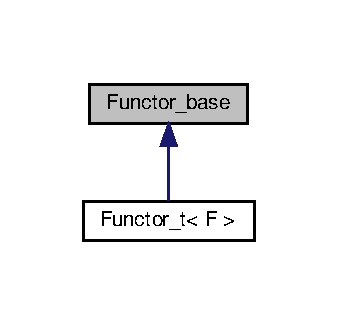
\includegraphics[width=162pt]{structFunctor__base__inherit__graph}
\end{center}
\end{figure}
\subsection*{Public 成员函数}
\begin{DoxyCompactItemize}
\item 
\mbox{\Hypertarget{structFunctor__base_a249b2f421002975fa78a41ec349e53bf}\label{structFunctor__base_a249b2f421002975fa78a41ec349e53bf}} 
virtual void {\bfseries call} ()=0
\end{DoxyCompactItemize}


\subsection{详细描述}
函数包装器虚基类 

该结构体的文档由以下文件生成\+:\begin{DoxyCompactItemize}
\item 
functor\+\_\+wrapper.\+hpp\end{DoxyCompactItemize}

\hypertarget{structFunctor__t}{}\section{Functor\+\_\+t$<$ F $>$ 模板结构体 参考}
\label{structFunctor__t}\index{Functor\+\_\+t$<$ F $>$@{Functor\+\_\+t$<$ F $>$}}


类 Functor\+\_\+t$<$ F $>$ 继承关系图\+:
\nopagebreak
\begin{figure}[H]
\begin{center}
\leavevmode
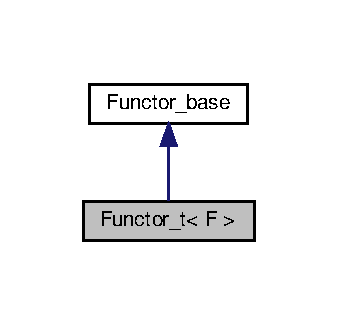
\includegraphics[width=162pt]{structFunctor__t__inherit__graph}
\end{center}
\end{figure}


Functor\+\_\+t$<$ F $>$ 的协作图\+:
\nopagebreak
\begin{figure}[H]
\begin{center}
\leavevmode
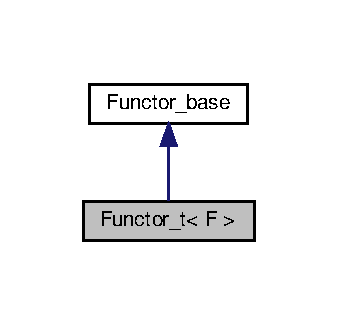
\includegraphics[width=162pt]{structFunctor__t__coll__graph}
\end{center}
\end{figure}
\subsection*{Public 成员函数}
\begin{DoxyCompactItemize}
\item 
\hyperlink{structFunctor__t_a1e788b8c1022f99a0e80b334b31383a2}{Functor\+\_\+t} (F \&\&f)
\begin{DoxyCompactList}\small\item\em functor\+\_\+t 构造函数 \end{DoxyCompactList}\item 
\mbox{\Hypertarget{structFunctor__t_ab4fc359c4f5955cc2d6a86214a5545ce}\label{structFunctor__t_ab4fc359c4f5955cc2d6a86214a5545ce}} 
void \hyperlink{structFunctor__t_ab4fc359c4f5955cc2d6a86214a5545ce}{call} () override
\begin{DoxyCompactList}\small\item\em call 执行被包装的函数 \end{DoxyCompactList}\end{DoxyCompactItemize}
\subsection*{Public 属性}
\begin{DoxyCompactItemize}
\item 
\mbox{\Hypertarget{structFunctor__t_a3fe63a336dc5daebf87bdc39090caa7a}\label{structFunctor__t_a3fe63a336dc5daebf87bdc39090caa7a}} 
F {\bfseries f\+\_\+}
\end{DoxyCompactItemize}


\subsection{构造及析构函数说明}
\mbox{\Hypertarget{structFunctor__t_a1e788b8c1022f99a0e80b334b31383a2}\label{structFunctor__t_a1e788b8c1022f99a0e80b334b31383a2}} 
\index{Functor\+\_\+t@{Functor\+\_\+t}!Functor\+\_\+t@{Functor\+\_\+t}}
\index{Functor\+\_\+t@{Functor\+\_\+t}!Functor\+\_\+t@{Functor\+\_\+t}}
\subsubsection{\texorpdfstring{Functor\+\_\+t()}{Functor\_t()}}
{\footnotesize\ttfamily template$<$typename F $>$ \\
\hyperlink{structFunctor__t}{Functor\+\_\+t}$<$ F $>$\+::\hyperlink{structFunctor__t}{Functor\+\_\+t} (\begin{DoxyParamCaption}\item[{F \&\&}]{f }\end{DoxyParamCaption})\hspace{0.3cm}{\ttfamily [inline]}}



functor\+\_\+t 构造函数 


\begin{DoxyParams}{参数}
{\em std\+::move(f)} & 包装的函数 \\
\hline
\end{DoxyParams}


该结构体的文档由以下文件生成\+:\begin{DoxyCompactItemize}
\item 
functor\+\_\+wrapper.\+hpp\end{DoxyCompactItemize}

\hypertarget{classRejectedExecutionHandler}{}\section{Rejected\+Execution\+Handler类 参考}
\label{classRejectedExecutionHandler}\index{Rejected\+Execution\+Handler@{Rejected\+Execution\+Handler}}


不再接受任务时的拒绝策略  




{\ttfamily \#include $<$threadpoolexecutor.\+hpp$>$}

\subsection*{Public 成员函数}
\begin{DoxyCompactItemize}
\item 
\mbox{\Hypertarget{classRejectedExecutionHandler_abb6476c7d64a7bd3111fc1a39829858b}\label{classRejectedExecutionHandler_abb6476c7d64a7bd3111fc1a39829858b}} 
virtual void {\bfseries rejected\+Execution} (const \hyperlink{classRunnable}{Runnable} \&r)
\end{DoxyCompactItemize}


\subsection{详细描述}
不再接受任务时的拒绝策略 

该类的文档由以下文件生成\+:\begin{DoxyCompactItemize}
\item 
threadpoolexecutor.\+hpp\end{DoxyCompactItemize}

\hypertarget{classRunnable}{}\section{Runnable类 参考}
\label{classRunnable}\index{Runnable@{Runnable}}


\hyperlink{classRunnable}{Runnable} interface 需要重写operator()  




{\ttfamily \#include $<$runnable.\+hpp$>$}

\subsection*{Public 成员函数}
\begin{DoxyCompactItemize}
\item 
\mbox{\Hypertarget{classRunnable_ab052afa8b53dd1e7c28e978962839446}\label{classRunnable_ab052afa8b53dd1e7c28e978962839446}} 
{\footnotesize template$<$typename F $>$ }\\{\bfseries Runnable} (F \&\&f)
\item 
\mbox{\Hypertarget{classRunnable_aaac34b8a861ab506499f8ec791e7cc16}\label{classRunnable_aaac34b8a861ab506499f8ec791e7cc16}} 
{\footnotesize template$<$typename F $>$ }\\{\bfseries Runnable} (F \&f)
\item 
\mbox{\Hypertarget{classRunnable_af028c95562f219c2af2439ae69e44755}\label{classRunnable_af028c95562f219c2af2439ae69e44755}} 
{\bfseries Runnable} (\hyperlink{classRunnable}{Runnable} \&\&other)
\item 
\mbox{\Hypertarget{classRunnable_a316ac005c1584a21b458fc673c04aed8}\label{classRunnable_a316ac005c1584a21b458fc673c04aed8}} 
{\bfseries Runnable} (const \hyperlink{classRunnable}{Runnable} \&other)
\item 
\mbox{\Hypertarget{classRunnable_a3ee19e0ee460449458ca79274908aef3}\label{classRunnable_a3ee19e0ee460449458ca79274908aef3}} 
\hyperlink{classRunnable}{Runnable} \& {\bfseries operator=} (\hyperlink{classRunnable}{Runnable} \&\&other)
\item 
\mbox{\Hypertarget{classRunnable_aac70062e7bc1f55cc1695fa37d75df53}\label{classRunnable_aac70062e7bc1f55cc1695fa37d75df53}} 
\hyperlink{classRunnable}{Runnable} \& {\bfseries operator=} (const \hyperlink{classRunnable}{Runnable} \&other)
\item 
\mbox{\Hypertarget{classRunnable_a38bf849dab4bbb86fc5bc6e7aff383e0}\label{classRunnable_a38bf849dab4bbb86fc5bc6e7aff383e0}} 
virtual void {\bfseries operator()} ()
\end{DoxyCompactItemize}


\subsection{详细描述}
\hyperlink{classRunnable}{Runnable} interface 需要重写operator() 

该类的文档由以下文件生成\+:\begin{DoxyCompactItemize}
\item 
runnable.\+hpp\end{DoxyCompactItemize}

\hypertarget{classRWLock}{}\section{R\+W\+Lock类 参考}
\label{classRWLock}\index{R\+W\+Lock@{R\+W\+Lock}}
\subsection*{Public 成员函数}
\begin{DoxyCompactItemize}
\item 
\mbox{\Hypertarget{classRWLock_a1ccd8fe0bf4931521e08df92f4662b2a}\label{classRWLock_a1ccd8fe0bf4931521e08df92f4662b2a}} 
int {\bfseries rd\+Lock} ()
\item 
\mbox{\Hypertarget{classRWLock_a6b034d61e35cce6702f284110f33ebdb}\label{classRWLock_a6b034d61e35cce6702f284110f33ebdb}} 
int {\bfseries wr\+Lock} ()
\item 
\mbox{\Hypertarget{classRWLock_ace8dce3640aa69fac39229a1096f064f}\label{classRWLock_ace8dce3640aa69fac39229a1096f064f}} 
int {\bfseries unlock} ()
\item 
\mbox{\Hypertarget{classRWLock_add87a7653a66092f1584fba8e3d75bc2}\label{classRWLock_add87a7653a66092f1584fba8e3d75bc2}} 
int {\bfseries try\+Rd\+Lock} ()
\item 
\mbox{\Hypertarget{classRWLock_a6a1b5fddaede8469cd774f20a93d7136}\label{classRWLock_a6a1b5fddaede8469cd774f20a93d7136}} 
int {\bfseries try\+Wr\+Lock} ()
\end{DoxyCompactItemize}


该类的文档由以下文件生成\+:\begin{DoxyCompactItemize}
\item 
rwlock.\+hpp\end{DoxyCompactItemize}

\hypertarget{classScheduledThreadPoolExecutor}{}\section{Scheduled\+Thread\+Pool\+Executor类 参考}
\label{classScheduledThreadPoolExecutor}\index{Scheduled\+Thread\+Pool\+Executor@{Scheduled\+Thread\+Pool\+Executor}}


定时任务调度线程池  




{\ttfamily \#include $<$scheduledthreadpoolexecutor.\+hpp$>$}



类 Scheduled\+Thread\+Pool\+Executor 继承关系图\+:\nopagebreak
\begin{figure}[H]
\begin{center}
\leavevmode
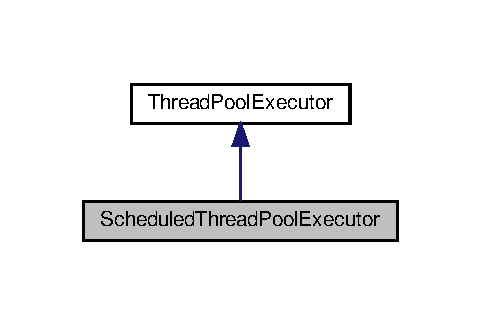
\includegraphics[width=231pt]{classScheduledThreadPoolExecutor__inherit__graph}
\end{center}
\end{figure}


Scheduled\+Thread\+Pool\+Executor 的协作图\+:\nopagebreak
\begin{figure}[H]
\begin{center}
\leavevmode
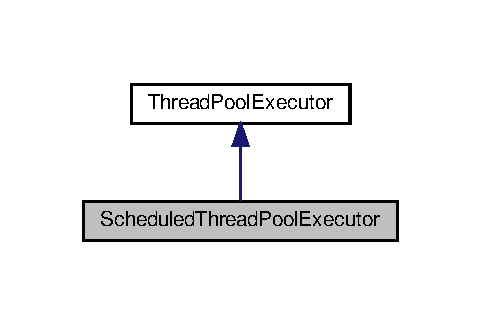
\includegraphics[width=231pt]{classScheduledThreadPoolExecutor__coll__graph}
\end{center}
\end{figure}
\subsection*{Public 成员函数}
\begin{DoxyCompactItemize}
\item 
\hyperlink{classScheduledThreadPoolExecutor_a880b17439bcdcf9b7542925e24033691}{Scheduled\+Thread\+Pool\+Executor} (int core\+Pool\+Size, const std\+::string \&prefix=\char`\"{}\char`\"{})
\begin{DoxyCompactList}\small\item\em \hyperlink{classScheduledThreadPoolExecutor}{Scheduled\+Thread\+Pool\+Executor} 构造函数 \end{DoxyCompactList}\item 
\mbox{\Hypertarget{classScheduledThreadPoolExecutor_aa8d3f9083aa92b351be6e134d7a675ea}\label{classScheduledThreadPoolExecutor_aa8d3f9083aa92b351be6e134d7a675ea}} 
virtual \hyperlink{classScheduledThreadPoolExecutor_aa8d3f9083aa92b351be6e134d7a675ea}{$\sim$\+Scheduled\+Thread\+Pool\+Executor} ()=default
\begin{DoxyCompactList}\small\item\em $\sim$\+Scheduled\+Thread\+Pool\+Executor 析构函数 \end{DoxyCompactList}\item 
\mbox{\Hypertarget{classScheduledThreadPoolExecutor_aabb4dbe81086385fb97cfa2a5d838dc8}\label{classScheduledThreadPoolExecutor_aabb4dbe81086385fb97cfa2a5d838dc8}} 
void {\bfseries execute} ()=delete
\item 
{\footnotesize template$<$typename F $>$ }\\void \hyperlink{classScheduledThreadPoolExecutor_a45e622833714db87a86d50eb45c8f338}{schedule} (F f, const std\+::chrono\+::nanoseconds \&delay)
\begin{DoxyCompactList}\small\item\em schedule 在将来某个时候执行给定的任务, 任务可以在新线程或现有的合并的线程中执行, 会抛出异常 \end{DoxyCompactList}\item 
void \hyperlink{classScheduledThreadPoolExecutor_a30f723414e619a950f1efd968d13921d}{schedule} (const std\+::shared\+\_\+ptr$<$ \hyperlink{structTimerTask}{Timer\+Task} $>$ \&f)
\begin{DoxyCompactList}\small\item\em schedule 在将来某个时候执行给定的任务, 任务可以在新线程或现有的合并的线程中执行, 会抛出异常 \end{DoxyCompactList}\item 
{\footnotesize template$<$typename F $>$ }\\void \hyperlink{classScheduledThreadPoolExecutor_aebcb96fcb3f5bfc6e55ffcef9f38d60b}{schedule\+At\+Fixed\+Rate} (F f, const std\+::chrono\+::nanoseconds \&initial\+Delay, const std\+::chrono\+::nanoseconds \&period)
\begin{DoxyCompactList}\small\item\em schedule\+At\+Fixed\+Rate 固定间隔调用 \end{DoxyCompactList}\item 
{\footnotesize template$<$typename F $>$ }\\void \hyperlink{classScheduledThreadPoolExecutor_a594bb3111f9d051ad12f366a13a54db0}{schedule\+At\+Fixed\+Delay} (F f, const std\+::chrono\+::nanoseconds \&initial\+Delay, const std\+::chrono\+::nanoseconds \&delay)
\begin{DoxyCompactList}\small\item\em schedule\+At\+Fixed\+Delay 固定延迟调用 \end{DoxyCompactList}\item 
virtual int \hyperlink{classScheduledThreadPoolExecutor_aed48379bdc243fd07e593205ca28f48d}{pre\+Start\+Core\+Threads} ()
\begin{DoxyCompactList}\small\item\em pre\+Start\+Core\+Threads 提前启动核心线程 \end{DoxyCompactList}\end{DoxyCompactItemize}
\subsection*{额外继承的成员函数}


\subsection{详细描述}
定时任务调度线程池 

\subsection{构造及析构函数说明}
\mbox{\Hypertarget{classScheduledThreadPoolExecutor_a880b17439bcdcf9b7542925e24033691}\label{classScheduledThreadPoolExecutor_a880b17439bcdcf9b7542925e24033691}} 
\index{Scheduled\+Thread\+Pool\+Executor@{Scheduled\+Thread\+Pool\+Executor}!Scheduled\+Thread\+Pool\+Executor@{Scheduled\+Thread\+Pool\+Executor}}
\index{Scheduled\+Thread\+Pool\+Executor@{Scheduled\+Thread\+Pool\+Executor}!Scheduled\+Thread\+Pool\+Executor@{Scheduled\+Thread\+Pool\+Executor}}
\subsubsection{\texorpdfstring{Scheduled\+Thread\+Pool\+Executor()}{ScheduledThreadPoolExecutor()}}
{\footnotesize\ttfamily Scheduled\+Thread\+Pool\+Executor\+::\+Scheduled\+Thread\+Pool\+Executor (\begin{DoxyParamCaption}\item[{int}]{core\+Pool\+Size,  }\item[{const std\+::string \&}]{prefix = {\ttfamily \char`\"{}\char`\"{}} }\end{DoxyParamCaption})\hspace{0.3cm}{\ttfamily [inline]}}



\hyperlink{classScheduledThreadPoolExecutor}{Scheduled\+Thread\+Pool\+Executor} 构造函数 


\begin{DoxyParams}{参数}
{\em core\+Pool\+Size} & 核心线程数量 \\
\hline
{\em prefix} & 线程名前缀 \\
\hline
\end{DoxyParams}


\subsection{成员函数说明}
\mbox{\Hypertarget{classScheduledThreadPoolExecutor_aed48379bdc243fd07e593205ca28f48d}\label{classScheduledThreadPoolExecutor_aed48379bdc243fd07e593205ca28f48d}} 
\index{Scheduled\+Thread\+Pool\+Executor@{Scheduled\+Thread\+Pool\+Executor}!pre\+Start\+Core\+Threads@{pre\+Start\+Core\+Threads}}
\index{pre\+Start\+Core\+Threads@{pre\+Start\+Core\+Threads}!Scheduled\+Thread\+Pool\+Executor@{Scheduled\+Thread\+Pool\+Executor}}
\subsubsection{\texorpdfstring{pre\+Start\+Core\+Threads()}{preStartCoreThreads()}}
{\footnotesize\ttfamily virtual int Scheduled\+Thread\+Pool\+Executor\+::pre\+Start\+Core\+Threads (\begin{DoxyParamCaption}{ }\end{DoxyParamCaption})\hspace{0.3cm}{\ttfamily [inline]}, {\ttfamily [virtual]}}



pre\+Start\+Core\+Threads 提前启动核心线程 

\begin{DoxyReturn}{返回}

\end{DoxyReturn}


重载 \hyperlink{classThreadPoolExecutor_aab8b3946a87fbecd144b159c12c8bcfb}{Thread\+Pool\+Executor} .

\mbox{\Hypertarget{classScheduledThreadPoolExecutor_a45e622833714db87a86d50eb45c8f338}\label{classScheduledThreadPoolExecutor_a45e622833714db87a86d50eb45c8f338}} 
\index{Scheduled\+Thread\+Pool\+Executor@{Scheduled\+Thread\+Pool\+Executor}!schedule@{schedule}}
\index{schedule@{schedule}!Scheduled\+Thread\+Pool\+Executor@{Scheduled\+Thread\+Pool\+Executor}}
\subsubsection{\texorpdfstring{schedule()}{schedule()}\hspace{0.1cm}{\footnotesize\ttfamily [1/2]}}
{\footnotesize\ttfamily template$<$typename F $>$ \\
void Scheduled\+Thread\+Pool\+Executor\+::schedule (\begin{DoxyParamCaption}\item[{F}]{f,  }\item[{const std\+::chrono\+::nanoseconds \&}]{delay }\end{DoxyParamCaption})\hspace{0.3cm}{\ttfamily [inline]}}



schedule 在将来某个时候执行给定的任务, 任务可以在新线程或现有的合并的线程中执行, 会抛出异常 


\begin{DoxyParams}{参数}
{\em f} & 要提交的任务(Runnable或函数或lambda,不能是\+Runnable\+::sptr) \\
\hline
{\em delay} & 固定延迟 \\
\hline
\end{DoxyParams}
\mbox{\Hypertarget{classScheduledThreadPoolExecutor_a30f723414e619a950f1efd968d13921d}\label{classScheduledThreadPoolExecutor_a30f723414e619a950f1efd968d13921d}} 
\index{Scheduled\+Thread\+Pool\+Executor@{Scheduled\+Thread\+Pool\+Executor}!schedule@{schedule}}
\index{schedule@{schedule}!Scheduled\+Thread\+Pool\+Executor@{Scheduled\+Thread\+Pool\+Executor}}
\subsubsection{\texorpdfstring{schedule()}{schedule()}\hspace{0.1cm}{\footnotesize\ttfamily [2/2]}}
{\footnotesize\ttfamily void Scheduled\+Thread\+Pool\+Executor\+::schedule (\begin{DoxyParamCaption}\item[{const std\+::shared\+\_\+ptr$<$ \hyperlink{structTimerTask}{Timer\+Task} $>$ \&}]{f }\end{DoxyParamCaption})\hspace{0.3cm}{\ttfamily [inline]}}



schedule 在将来某个时候执行给定的任务, 任务可以在新线程或现有的合并的线程中执行, 会抛出异常 


\begin{DoxyParams}{参数}
{\em f} & 要提交的任务(std\+::shared\+\_\+ptr$<$\+Timer\+Task$>$) \\
\hline
\end{DoxyParams}
\mbox{\Hypertarget{classScheduledThreadPoolExecutor_a594bb3111f9d051ad12f366a13a54db0}\label{classScheduledThreadPoolExecutor_a594bb3111f9d051ad12f366a13a54db0}} 
\index{Scheduled\+Thread\+Pool\+Executor@{Scheduled\+Thread\+Pool\+Executor}!schedule\+At\+Fixed\+Delay@{schedule\+At\+Fixed\+Delay}}
\index{schedule\+At\+Fixed\+Delay@{schedule\+At\+Fixed\+Delay}!Scheduled\+Thread\+Pool\+Executor@{Scheduled\+Thread\+Pool\+Executor}}
\subsubsection{\texorpdfstring{schedule\+At\+Fixed\+Delay()}{scheduleAtFixedDelay()}}
{\footnotesize\ttfamily template$<$typename F $>$ \\
void Scheduled\+Thread\+Pool\+Executor\+::schedule\+At\+Fixed\+Delay (\begin{DoxyParamCaption}\item[{F}]{f,  }\item[{const std\+::chrono\+::nanoseconds \&}]{initial\+Delay,  }\item[{const std\+::chrono\+::nanoseconds \&}]{delay }\end{DoxyParamCaption})\hspace{0.3cm}{\ttfamily [inline]}}



schedule\+At\+Fixed\+Delay 固定延迟调用 


\begin{DoxyParams}{参数}
{\em f} & 要提交的任务(Runnable或函数或lambda,不能是\+Runnable\+::sptr) \\
\hline
{\em initial\+Delay} & 初始延迟 \\
\hline
{\em delay} & 固定延迟 \\
\hline
\end{DoxyParams}
\mbox{\Hypertarget{classScheduledThreadPoolExecutor_aebcb96fcb3f5bfc6e55ffcef9f38d60b}\label{classScheduledThreadPoolExecutor_aebcb96fcb3f5bfc6e55ffcef9f38d60b}} 
\index{Scheduled\+Thread\+Pool\+Executor@{Scheduled\+Thread\+Pool\+Executor}!schedule\+At\+Fixed\+Rate@{schedule\+At\+Fixed\+Rate}}
\index{schedule\+At\+Fixed\+Rate@{schedule\+At\+Fixed\+Rate}!Scheduled\+Thread\+Pool\+Executor@{Scheduled\+Thread\+Pool\+Executor}}
\subsubsection{\texorpdfstring{schedule\+At\+Fixed\+Rate()}{scheduleAtFixedRate()}}
{\footnotesize\ttfamily template$<$typename F $>$ \\
void Scheduled\+Thread\+Pool\+Executor\+::schedule\+At\+Fixed\+Rate (\begin{DoxyParamCaption}\item[{F}]{f,  }\item[{const std\+::chrono\+::nanoseconds \&}]{initial\+Delay,  }\item[{const std\+::chrono\+::nanoseconds \&}]{period }\end{DoxyParamCaption})\hspace{0.3cm}{\ttfamily [inline]}}



schedule\+At\+Fixed\+Rate 固定间隔调用 


\begin{DoxyParams}{参数}
{\em f} & 要提交的任务(Runnable或函数或lambda,不能是\+Runnable\+::sptr) \\
\hline
{\em initial\+Delay} & 初始延迟 \\
\hline
{\em period} & 固定间隔 \\
\hline
\end{DoxyParams}


该类的文档由以下文件生成\+:\begin{DoxyCompactItemize}
\item 
scheduledthreadpoolexecutor.\+hpp\end{DoxyCompactItemize}

\hypertarget{classSemaphore}{}\section{Semaphore类 参考}
\label{classSemaphore}\index{Semaphore@{Semaphore}}


信号量  




{\ttfamily \#include $<$semaphore.\+hpp$>$}

\subsection*{Public 成员函数}
\begin{DoxyCompactItemize}
\item 
int \hyperlink{classSemaphore_a93794b9ab0c6c7c35acce0769bf67caf}{post} ()
\begin{DoxyCompactList}\small\item\em post 信号量加一 \end{DoxyCompactList}\item 
int \hyperlink{classSemaphore_ab50da3ab3fdc7f56acc85cbdf248c98d}{wait} ()
\begin{DoxyCompactList}\small\item\em wait 信号量减一 \end{DoxyCompactList}\item 
int \hyperlink{classSemaphore_acc15178e43d33745f4acc6e2b2cccf9b}{try\+Wait} ()
\begin{DoxyCompactList}\small\item\em try\+Wait 信号量减一,立即返回 \end{DoxyCompactList}\item 
int \hyperlink{classSemaphore_a203e6b9f726ca5defc94379e9145278e}{timed\+Wait} (unsigned int seconds, unsigned int nanoseconds)
\begin{DoxyCompactList}\small\item\em timed\+Wait 信号量减一 \end{DoxyCompactList}\item 
\hyperlink{classSemaphore_a34841feb22e781d7d10ee7205f56bd8e}{Semaphore} (unsigned int init\+Size=0)
\begin{DoxyCompactList}\small\item\em \hyperlink{classSemaphore}{Semaphore} 构造函数 \end{DoxyCompactList}\item 
\mbox{\Hypertarget{classSemaphore_a7039839a61ed189258fb0de6338848e3}\label{classSemaphore_a7039839a61ed189258fb0de6338848e3}} 
virtual \hyperlink{classSemaphore_a7039839a61ed189258fb0de6338848e3}{$\sim$\+Semaphore} ()
\begin{DoxyCompactList}\small\item\em $\sim$\+Semaphore 析构函数 \end{DoxyCompactList}\item 
\mbox{\Hypertarget{classSemaphore_a89fbc8358ec2936a0f90bf7144c5f02a}\label{classSemaphore_a89fbc8358ec2936a0f90bf7144c5f02a}} 
{\bfseries Semaphore} (const \hyperlink{classSemaphore}{Semaphore} \&)=delete
\item 
\mbox{\Hypertarget{classSemaphore_abd3d859134189efbc4be845048dcda24}\label{classSemaphore_abd3d859134189efbc4be845048dcda24}} 
{\bfseries Semaphore} (const \hyperlink{classSemaphore}{Semaphore} \&\&)=delete
\item 
\mbox{\Hypertarget{classSemaphore_a807f887093da67cb0d4ad302850b9499}\label{classSemaphore_a807f887093da67cb0d4ad302850b9499}} 
\hyperlink{classSemaphore}{Semaphore} \& {\bfseries operator=} (const \hyperlink{classSemaphore}{Semaphore} \&)=delete
\item 
\mbox{\Hypertarget{classSemaphore_a453616a4ed5693d85c71df144999c4d3}\label{classSemaphore_a453616a4ed5693d85c71df144999c4d3}} 
\hyperlink{classSemaphore}{Semaphore} \& {\bfseries operator=} (const \hyperlink{classSemaphore}{Semaphore} \&\&)=delete
\end{DoxyCompactItemize}


\subsection{详细描述}
信号量 

\subsection{构造及析构函数说明}
\mbox{\Hypertarget{classSemaphore_a34841feb22e781d7d10ee7205f56bd8e}\label{classSemaphore_a34841feb22e781d7d10ee7205f56bd8e}} 
\index{Semaphore@{Semaphore}!Semaphore@{Semaphore}}
\index{Semaphore@{Semaphore}!Semaphore@{Semaphore}}
\subsubsection{\texorpdfstring{Semaphore()}{Semaphore()}}
{\footnotesize\ttfamily Semaphore\+::\+Semaphore (\begin{DoxyParamCaption}\item[{unsigned int}]{init\+Size = {\ttfamily 0} }\end{DoxyParamCaption})\hspace{0.3cm}{\ttfamily [inline]}}



\hyperlink{classSemaphore}{Semaphore} 构造函数 


\begin{DoxyParams}{参数}
{\em init\+Size} & 信号量初值 \\
\hline
\end{DoxyParams}


\subsection{成员函数说明}
\mbox{\Hypertarget{classSemaphore_a93794b9ab0c6c7c35acce0769bf67caf}\label{classSemaphore_a93794b9ab0c6c7c35acce0769bf67caf}} 
\index{Semaphore@{Semaphore}!post@{post}}
\index{post@{post}!Semaphore@{Semaphore}}
\subsubsection{\texorpdfstring{post()}{post()}}
{\footnotesize\ttfamily int Semaphore\+::post (\begin{DoxyParamCaption}{ }\end{DoxyParamCaption})\hspace{0.3cm}{\ttfamily [inline]}}



post 信号量加一 

\begin{DoxyReturn}{返回}
错误码 0表示成功 
\end{DoxyReturn}
\mbox{\Hypertarget{classSemaphore_a203e6b9f726ca5defc94379e9145278e}\label{classSemaphore_a203e6b9f726ca5defc94379e9145278e}} 
\index{Semaphore@{Semaphore}!timed\+Wait@{timed\+Wait}}
\index{timed\+Wait@{timed\+Wait}!Semaphore@{Semaphore}}
\subsubsection{\texorpdfstring{timed\+Wait()}{timedWait()}}
{\footnotesize\ttfamily int Semaphore\+::timed\+Wait (\begin{DoxyParamCaption}\item[{unsigned int}]{seconds,  }\item[{unsigned int}]{nanoseconds }\end{DoxyParamCaption})\hspace{0.3cm}{\ttfamily [inline]}}



timed\+Wait 信号量减一 


\begin{DoxyParams}{参数}
{\em seconds} & 等待时间-秒 \\
\hline
{\em nanoseconds} & 等待时间-纳秒\\
\hline
\end{DoxyParams}
\begin{DoxyReturn}{返回}
错误码 0表示成功 
\end{DoxyReturn}
\mbox{\Hypertarget{classSemaphore_acc15178e43d33745f4acc6e2b2cccf9b}\label{classSemaphore_acc15178e43d33745f4acc6e2b2cccf9b}} 
\index{Semaphore@{Semaphore}!try\+Wait@{try\+Wait}}
\index{try\+Wait@{try\+Wait}!Semaphore@{Semaphore}}
\subsubsection{\texorpdfstring{try\+Wait()}{tryWait()}}
{\footnotesize\ttfamily int Semaphore\+::try\+Wait (\begin{DoxyParamCaption}{ }\end{DoxyParamCaption})\hspace{0.3cm}{\ttfamily [inline]}}



try\+Wait 信号量减一,立即返回 

\begin{DoxyReturn}{返回}
错误码 0表示成功 
\end{DoxyReturn}
\mbox{\Hypertarget{classSemaphore_ab50da3ab3fdc7f56acc85cbdf248c98d}\label{classSemaphore_ab50da3ab3fdc7f56acc85cbdf248c98d}} 
\index{Semaphore@{Semaphore}!wait@{wait}}
\index{wait@{wait}!Semaphore@{Semaphore}}
\subsubsection{\texorpdfstring{wait()}{wait()}}
{\footnotesize\ttfamily int Semaphore\+::wait (\begin{DoxyParamCaption}{ }\end{DoxyParamCaption})\hspace{0.3cm}{\ttfamily [inline]}}



wait 信号量减一 

\begin{DoxyReturn}{返回}
错误码 0表示成功 
\end{DoxyReturn}


该类的文档由以下文件生成\+:\begin{DoxyCompactItemize}
\item 
semaphore.\+hpp\end{DoxyCompactItemize}

\hypertarget{classThread}{}\section{Thread类 参考}
\label{classThread}\index{Thread@{Thread}}
\subsection*{类}
\begin{DoxyCompactItemize}
\item 
struct \hyperlink{structThread_1_1Func__base}{Func\+\_\+base}
\item 
struct \hyperlink{structThread_1_1Func__t}{Func\+\_\+t}
\end{DoxyCompactItemize}
\subsection*{Public 类型}
\begin{DoxyCompactItemize}
\item 
\mbox{\Hypertarget{classThread_a430059e402325caaf1ed185fb520c9d2}\label{classThread_a430059e402325caaf1ed185fb520c9d2}} 
using {\bfseries sptr} = std\+::shared\+\_\+ptr$<$ \hyperlink{classThread}{Thread} $>$
\end{DoxyCompactItemize}
\subsection*{Public 成员函数}
\begin{DoxyCompactItemize}
\item 
\hyperlink{classThread_a2375aeb8a227668652d593b180bac64e}{Thread} (int pro, \hyperlink{classThreadPoolExecutor}{Thread\+Pool\+Executor} $\ast$tpe=nullptr)
\begin{DoxyCompactList}\small\item\em \hyperlink{classThread}{Thread} 构造函数 \end{DoxyCompactList}\item 
\hyperlink{classThread_aa32c32f43d92d235c9e795bea80e9058}{Thread} (const std\+::string \&name=\char`\"{}\char`\"{}, int pro=20, \hyperlink{classThreadPoolExecutor}{Thread\+Pool\+Executor} $\ast$tpe=nullptr)
\begin{DoxyCompactList}\small\item\em \hyperlink{classThread}{Thread} 构造函数 \end{DoxyCompactList}\item 
{\footnotesize template$<$typename Function\+Type $>$ }\\\hyperlink{classThread_a67eed36a7c4cb621651a6ce40939cf44}{Thread} (Function\+Type f, const std\+::string \&name=\char`\"{}\char`\"{}, int pro=20, \hyperlink{classThreadPoolExecutor}{Thread\+Pool\+Executor} $\ast$tpe=nullptr)
\begin{DoxyCompactList}\small\item\em \hyperlink{classThread}{Thread} 构造函数 \end{DoxyCompactList}\item 
\mbox{\Hypertarget{classThread_a957c601b090d6c2798c3cceb4ae5dc0f}\label{classThread_a957c601b090d6c2798c3cceb4ae5dc0f}} 
virtual \hyperlink{classThread_a957c601b090d6c2798c3cceb4ae5dc0f}{$\sim$\+Thread} ()=default
\begin{DoxyCompactList}\small\item\em $\sim$\+Thread 析构函数 \end{DoxyCompactList}\item 
\mbox{\Hypertarget{classThread_a3a36451e02a15180624cdd88212cb1ba}\label{classThread_a3a36451e02a15180624cdd88212cb1ba}} 
virtual void \hyperlink{classThread_a3a36451e02a15180624cdd88212cb1ba}{start} () final
\begin{DoxyCompactList}\small\item\em start 开始执行线程,如果构造函数传入了\+Func, 那么重写的run方法不会执行 \end{DoxyCompactList}\item 
\mbox{\Hypertarget{classThread_a07b23d8d75300651cba3eb79652c77fd}\label{classThread_a07b23d8d75300651cba3eb79652c77fd}} 
virtual void \hyperlink{classThread_a07b23d8d75300651cba3eb79652c77fd}{join} () final
\begin{DoxyCompactList}\small\item\em join 释放线程资源 \end{DoxyCompactList}\item 
\mbox{\Hypertarget{classThread_affb34b8590eab79785627ae48cbd297d}\label{classThread_affb34b8590eab79785627ae48cbd297d}} 
virtual void \hyperlink{classThread_affb34b8590eab79785627ae48cbd297d}{detach} () final
\begin{DoxyCompactList}\small\item\em detach 释放线程 \end{DoxyCompactList}\item 
\mbox{\Hypertarget{classThread_ac09e8b8ff4fb0a97315b5a501e722783}\label{classThread_ac09e8b8ff4fb0a97315b5a501e722783}} 
virtual void \hyperlink{classThread_ac09e8b8ff4fb0a97315b5a501e722783}{yield} () final
\begin{DoxyCompactList}\small\item\em yield 让出时间片 \end{DoxyCompactList}\item 
virtual bool \hyperlink{classThread_a86d1c278c0b9fea63037c437a909064f}{joinable} () const final
\begin{DoxyCompactList}\small\item\em joinable \end{DoxyCompactList}\item 
virtual std\+::thread\+::native\+\_\+handle\+\_\+type \hyperlink{classThread_a554185abbfacbcc4bf2e953cdddcbbba}{self} () final
\begin{DoxyCompactList}\small\item\em self 返回线程底层句柄 \end{DoxyCompactList}\item 
virtual std\+::string \hyperlink{classThread_a19bc237f8a86727a5a4b516122fe20f6}{get\+Name} () const final
\begin{DoxyCompactList}\small\item\em get\+Name 得到线程名称 \end{DoxyCompactList}\item 
virtual void \hyperlink{classThread_ae816904b2a3e248472813e17c2b12a71}{set\+Name} (const std\+::string \&name) final
\begin{DoxyCompactList}\small\item\em set\+Name 设置线程名称 \end{DoxyCompactList}\item 
virtual pid\+\_\+t \hyperlink{classThread_a2940721084b607bbc2981e8754ea2d9c}{get\+Current\+Pid} () const final
\begin{DoxyCompactList}\small\item\em get\+Current\+Pid 获取\+Linux底层线程id, start之后才有效,-\/1表示线程已经结束 \end{DoxyCompactList}\item 
virtual std\+::chrono\+::steady\+\_\+clock\+::time\+\_\+point \hyperlink{classThread_a23de6830557bdbe18a0baf17db58aec6}{get\+Last\+Active\+Time} () const final
\begin{DoxyCompactList}\small\item\em get\+Last\+Active\+Time 上一次活跃时间 \end{DoxyCompactList}\item 
virtual uint64\+\_\+t \hyperlink{classThread_abe37a59eed637eebb11d4ce75f4d95c7}{unique\+Id} () const final
\begin{DoxyCompactList}\small\item\em unique\+Id 获取线程unique\+Id \end{DoxyCompactList}\item 
virtual std\+::thread\+::id \hyperlink{classThread_a231da16ab1825ee982c4aa43f78c1b22}{std\+Id} () final
\begin{DoxyCompactList}\small\item\em std\+Id 获取线程thread\+::id \end{DoxyCompactList}\item 
virtual bool \hyperlink{classThread_acb6c590deecea4778a855459f080060a}{is\+Idle} () const final
\begin{DoxyCompactList}\small\item\em is\+Idle 查看线程是否空闲,使用的是类内部成员变量,与is\+Running不同 \end{DoxyCompactList}\item 
virtual bool \hyperlink{classThread_ab4c718f3ca4aa7514c7e89e38f9da894}{is\+Running} () final
\begin{DoxyCompactList}\small\item\em is\+Running 查看线程是否还在运行,使用pthread\+\_\+kill向线程发信号 \end{DoxyCompactList}\item 
virtual void \hyperlink{classThread_a96661f80f5fbd26042a24eafd675cd91}{set\+Prio} (int prio) final
\begin{DoxyCompactList}\small\item\em set\+Prio 设置优先级 \end{DoxyCompactList}\item 
virtual int \hyperlink{classThread_a712ab58b9e89f458427b213b1197a666}{get\+Prio} () final
\begin{DoxyCompactList}\small\item\em get\+Prio 获取线程优先级 \end{DoxyCompactList}\item 
\mbox{\Hypertarget{classThread_a9c8be569889e6acc065a9db76f738952}\label{classThread_a9c8be569889e6acc065a9db76f738952}} 
{\bfseries Thread} (const \hyperlink{classThread}{Thread} \&\&)=delete
\item 
\mbox{\Hypertarget{classThread_ab6968c245fad4970965b3bf9f6027642}\label{classThread_ab6968c245fad4970965b3bf9f6027642}} 
\hyperlink{classThread}{Thread} \& {\bfseries operator=} (const \hyperlink{classThread}{Thread} \&\&)=delete
\item 
\mbox{\Hypertarget{classThread_a71c9b9c8fb2e87eb14279f6233a83143}\label{classThread_a71c9b9c8fb2e87eb14279f6233a83143}} 
{\bfseries Thread} (const \hyperlink{classThread}{Thread} \&)=delete
\item 
\mbox{\Hypertarget{classThread_a832b2ddff787923f27430d95df55c83d}\label{classThread_a832b2ddff787923f27430d95df55c83d}} 
\hyperlink{classThread}{Thread} \& {\bfseries operator=} (const \hyperlink{classThread}{Thread} \&)=delete
\end{DoxyCompactItemize}
\subsection*{静态 Public 成员函数}
\begin{DoxyCompactItemize}
\item 
\mbox{\Hypertarget{classThread_a7e6f38efc79df2e36e0ac9e0f7c1a833}\label{classThread_a7e6f38efc79df2e36e0ac9e0f7c1a833}} 
static int {\bfseries get\+Next\+Id} ()
\end{DoxyCompactItemize}
\subsection*{Protected 属性}
\begin{DoxyCompactItemize}
\item 
\mbox{\Hypertarget{classThread_a23541f34356cb161bb5fe6026bb3000a}\label{classThread_a23541f34356cb161bb5fe6026bb3000a}} 
bool {\bfseries idle\+\_\+} \{true\}
\item 
\mbox{\Hypertarget{classThread_ada8c342b34fb001cfcf57619b7150840}\label{classThread_ada8c342b34fb001cfcf57619b7150840}} 
int {\bfseries prio\+\_\+}
\item 
\mbox{\Hypertarget{classThread_a0c0878a96696bbb092a69bc2f1f812fd}\label{classThread_a0c0878a96696bbb092a69bc2f1f812fd}} 
pid\+\_\+t {\bfseries current\+Pid\+\_\+} \{-\/1\}
\item 
\mbox{\Hypertarget{classThread_a6087bbfff90554d609fa22b4e4893afb}\label{classThread_a6087bbfff90554d609fa22b4e4893afb}} 
uint64\+\_\+t \hyperlink{classThread_a6087bbfff90554d609fa22b4e4893afb}{unique\+Id\+\_\+} \{next\+Id\+\_\+++\}
\begin{DoxyCompactList}\small\item\em -\/1表明线程已经执行完任务,unix底层的线程已经不存在了 \end{DoxyCompactList}\item 
\mbox{\Hypertarget{classThread_aa222eb32e5fc8f386d9fb018607acd9c}\label{classThread_aa222eb32e5fc8f386d9fb018607acd9c}} 
std\+::string \hyperlink{classThread_aa222eb32e5fc8f386d9fb018607acd9c}{name\+\_\+}
\begin{DoxyCompactList}\small\item\em 当前线程id与系统无关 \end{DoxyCompactList}\item 
\mbox{\Hypertarget{classThread_ad313ba812a7875c743dd0d37d565acfb}\label{classThread_ad313ba812a7875c743dd0d37d565acfb}} 
std\+::thread {\bfseries thread\+\_\+}
\item 
\mbox{\Hypertarget{classThread_ae8ebc3f208496db3052de7a56eb6e895}\label{classThread_ae8ebc3f208496db3052de7a56eb6e895}} 
std\+::atomic$<$ bool $>$ {\bfseries yield\+\_\+} \{false\}
\item 
\mbox{\Hypertarget{classThread_ae7ed71c6b1f7782ecd4186005fd70760}\label{classThread_ae7ed71c6b1f7782ecd4186005fd70760}} 
std\+::chrono\+::steady\+\_\+clock\+::time\+\_\+point {\bfseries last\+Active\+Time\+\_\+} \{std\+::chrono\+::steady\+\_\+clock\+::now()\}
\item 
\mbox{\Hypertarget{classThread_a677202a7d90ebc5a6d4f8b1eab1a1eac}\label{classThread_a677202a7d90ebc5a6d4f8b1eab1a1eac}} 
std\+::unique\+\_\+ptr$<$ \hyperlink{structThread_1_1Func__base}{Func\+\_\+base} $>$ {\bfseries func\+\_\+uptr\+\_\+}
\end{DoxyCompactItemize}
\subsection*{静态 Protected 属性}
\begin{DoxyCompactItemize}
\item 
\mbox{\Hypertarget{classThread_ab6f45a9de088d45853895ff98a5db0e8}\label{classThread_ab6f45a9de088d45853895ff98a5db0e8}} 
static std\+::atomic$<$ uint64\+\_\+t $>$ {\bfseries next\+Id\+\_\+}
\end{DoxyCompactItemize}


\subsection{构造及析构函数说明}
\mbox{\Hypertarget{classThread_a2375aeb8a227668652d593b180bac64e}\label{classThread_a2375aeb8a227668652d593b180bac64e}} 
\index{Thread@{Thread}!Thread@{Thread}}
\index{Thread@{Thread}!Thread@{Thread}}
\subsubsection{\texorpdfstring{Thread()}{Thread()}\hspace{0.1cm}{\footnotesize\ttfamily [1/3]}}
{\footnotesize\ttfamily Thread\+::\+Thread (\begin{DoxyParamCaption}\item[{int}]{pro,  }\item[{\hyperlink{classThreadPoolExecutor}{Thread\+Pool\+Executor} $\ast$}]{tpe = {\ttfamily nullptr} }\end{DoxyParamCaption})\hspace{0.3cm}{\ttfamily [inline]}}



\hyperlink{classThread}{Thread} 构造函数 


\begin{DoxyParams}{参数}
{\em pro} & 优先级 \\
\hline
{\em tpe} & 线程池(nullptr) \\
\hline
\end{DoxyParams}
\mbox{\Hypertarget{classThread_aa32c32f43d92d235c9e795bea80e9058}\label{classThread_aa32c32f43d92d235c9e795bea80e9058}} 
\index{Thread@{Thread}!Thread@{Thread}}
\index{Thread@{Thread}!Thread@{Thread}}
\subsubsection{\texorpdfstring{Thread()}{Thread()}\hspace{0.1cm}{\footnotesize\ttfamily [2/3]}}
{\footnotesize\ttfamily Thread\+::\+Thread (\begin{DoxyParamCaption}\item[{const std\+::string \&}]{name = {\ttfamily \char`\"{}\char`\"{}},  }\item[{int}]{pro = {\ttfamily 20},  }\item[{\hyperlink{classThreadPoolExecutor}{Thread\+Pool\+Executor} $\ast$}]{tpe = {\ttfamily nullptr} }\end{DoxyParamCaption})\hspace{0.3cm}{\ttfamily [inline]}}



\hyperlink{classThread}{Thread} 构造函数 


\begin{DoxyParams}{参数}
{\em name} & 线程名 \\
\hline
{\em pro} & 优先级 \\
\hline
{\em tpe} & 线程池(nullptr) \\
\hline
\end{DoxyParams}
\mbox{\Hypertarget{classThread_a67eed36a7c4cb621651a6ce40939cf44}\label{classThread_a67eed36a7c4cb621651a6ce40939cf44}} 
\index{Thread@{Thread}!Thread@{Thread}}
\index{Thread@{Thread}!Thread@{Thread}}
\subsubsection{\texorpdfstring{Thread()}{Thread()}\hspace{0.1cm}{\footnotesize\ttfamily [3/3]}}
{\footnotesize\ttfamily template$<$typename Function\+Type $>$ \\
Thread\+::\+Thread (\begin{DoxyParamCaption}\item[{Function\+Type}]{f,  }\item[{const std\+::string \&}]{name = {\ttfamily \char`\"{}\char`\"{}},  }\item[{int}]{pro = {\ttfamily 20},  }\item[{\hyperlink{classThreadPoolExecutor}{Thread\+Pool\+Executor} $\ast$}]{tpe = {\ttfamily nullptr} }\end{DoxyParamCaption})\hspace{0.3cm}{\ttfamily [inline]}}



\hyperlink{classThread}{Thread} 构造函数 


\begin{DoxyParams}{参数}
{\em f} & 要执行的任务 \\
\hline
{\em name} & 线程名 \\
\hline
{\em pro} & 优先级 \\
\hline
{\em tpe} & 线程池(nullptr) \\
\hline
\end{DoxyParams}


\subsection{成员函数说明}
\mbox{\Hypertarget{classThread_a2940721084b607bbc2981e8754ea2d9c}\label{classThread_a2940721084b607bbc2981e8754ea2d9c}} 
\index{Thread@{Thread}!get\+Current\+Pid@{get\+Current\+Pid}}
\index{get\+Current\+Pid@{get\+Current\+Pid}!Thread@{Thread}}
\subsubsection{\texorpdfstring{get\+Current\+Pid()}{getCurrentPid()}}
{\footnotesize\ttfamily virtual pid\+\_\+t Thread\+::get\+Current\+Pid (\begin{DoxyParamCaption}{ }\end{DoxyParamCaption}) const\hspace{0.3cm}{\ttfamily [inline]}, {\ttfamily [final]}, {\ttfamily [virtual]}}



get\+Current\+Pid 获取\+Linux底层线程id, start之后才有效,-\/1表示线程已经结束 

\begin{DoxyReturn}{返回}
pid\+\_\+t Linux底层线程id 
\end{DoxyReturn}
\mbox{\Hypertarget{classThread_a23de6830557bdbe18a0baf17db58aec6}\label{classThread_a23de6830557bdbe18a0baf17db58aec6}} 
\index{Thread@{Thread}!get\+Last\+Active\+Time@{get\+Last\+Active\+Time}}
\index{get\+Last\+Active\+Time@{get\+Last\+Active\+Time}!Thread@{Thread}}
\subsubsection{\texorpdfstring{get\+Last\+Active\+Time()}{getLastActiveTime()}}
{\footnotesize\ttfamily virtual std\+::chrono\+::steady\+\_\+clock\+::time\+\_\+point Thread\+::get\+Last\+Active\+Time (\begin{DoxyParamCaption}{ }\end{DoxyParamCaption}) const\hspace{0.3cm}{\ttfamily [inline]}, {\ttfamily [final]}, {\ttfamily [virtual]}}



get\+Last\+Active\+Time 上一次活跃时间 

\begin{DoxyReturn}{返回}
std\+::chrono\+::steady\+\_\+clock\+::time\+\_\+point 上一次活跃时间 
\end{DoxyReturn}
\mbox{\Hypertarget{classThread_a19bc237f8a86727a5a4b516122fe20f6}\label{classThread_a19bc237f8a86727a5a4b516122fe20f6}} 
\index{Thread@{Thread}!get\+Name@{get\+Name}}
\index{get\+Name@{get\+Name}!Thread@{Thread}}
\subsubsection{\texorpdfstring{get\+Name()}{getName()}}
{\footnotesize\ttfamily virtual std\+::string Thread\+::get\+Name (\begin{DoxyParamCaption}{ }\end{DoxyParamCaption}) const\hspace{0.3cm}{\ttfamily [inline]}, {\ttfamily [final]}, {\ttfamily [virtual]}}



get\+Name 得到线程名称 

\begin{DoxyReturn}{返回}
std\+::string name线程名称 
\end{DoxyReturn}
\mbox{\Hypertarget{classThread_a712ab58b9e89f458427b213b1197a666}\label{classThread_a712ab58b9e89f458427b213b1197a666}} 
\index{Thread@{Thread}!get\+Prio@{get\+Prio}}
\index{get\+Prio@{get\+Prio}!Thread@{Thread}}
\subsubsection{\texorpdfstring{get\+Prio()}{getPrio()}}
{\footnotesize\ttfamily virtual int Thread\+::get\+Prio (\begin{DoxyParamCaption}{ }\end{DoxyParamCaption})\hspace{0.3cm}{\ttfamily [inline]}, {\ttfamily [final]}, {\ttfamily [virtual]}}



get\+Prio 获取线程优先级 

\begin{DoxyReturn}{返回}
prio 优先级 
\end{DoxyReturn}
\mbox{\Hypertarget{classThread_acb6c590deecea4778a855459f080060a}\label{classThread_acb6c590deecea4778a855459f080060a}} 
\index{Thread@{Thread}!is\+Idle@{is\+Idle}}
\index{is\+Idle@{is\+Idle}!Thread@{Thread}}
\subsubsection{\texorpdfstring{is\+Idle()}{isIdle()}}
{\footnotesize\ttfamily virtual bool Thread\+::is\+Idle (\begin{DoxyParamCaption}{ }\end{DoxyParamCaption}) const\hspace{0.3cm}{\ttfamily [inline]}, {\ttfamily [final]}, {\ttfamily [virtual]}}



is\+Idle 查看线程是否空闲,使用的是类内部成员变量,与is\+Running不同 

\begin{DoxyReturn}{返回}
bool true-\/线程空闲 
\end{DoxyReturn}
\mbox{\Hypertarget{classThread_ab4c718f3ca4aa7514c7e89e38f9da894}\label{classThread_ab4c718f3ca4aa7514c7e89e38f9da894}} 
\index{Thread@{Thread}!is\+Running@{is\+Running}}
\index{is\+Running@{is\+Running}!Thread@{Thread}}
\subsubsection{\texorpdfstring{is\+Running()}{isRunning()}}
{\footnotesize\ttfamily virtual bool Thread\+::is\+Running (\begin{DoxyParamCaption}{ }\end{DoxyParamCaption})\hspace{0.3cm}{\ttfamily [inline]}, {\ttfamily [final]}, {\ttfamily [virtual]}}



is\+Running 查看线程是否还在运行,使用pthread\+\_\+kill向线程发信号 

\begin{DoxyReturn}{返回}
bool true-\/还在运行 
\end{DoxyReturn}
\mbox{\Hypertarget{classThread_a86d1c278c0b9fea63037c437a909064f}\label{classThread_a86d1c278c0b9fea63037c437a909064f}} 
\index{Thread@{Thread}!joinable@{joinable}}
\index{joinable@{joinable}!Thread@{Thread}}
\subsubsection{\texorpdfstring{joinable()}{joinable()}}
{\footnotesize\ttfamily virtual bool Thread\+::joinable (\begin{DoxyParamCaption}{ }\end{DoxyParamCaption}) const\hspace{0.3cm}{\ttfamily [inline]}, {\ttfamily [final]}, {\ttfamily [virtual]}}



joinable 

\begin{DoxyReturn}{返回}
bool 
\end{DoxyReturn}
\mbox{\Hypertarget{classThread_a554185abbfacbcc4bf2e953cdddcbbba}\label{classThread_a554185abbfacbcc4bf2e953cdddcbbba}} 
\index{Thread@{Thread}!self@{self}}
\index{self@{self}!Thread@{Thread}}
\subsubsection{\texorpdfstring{self()}{self()}}
{\footnotesize\ttfamily virtual std\+::thread\+::native\+\_\+handle\+\_\+type Thread\+::self (\begin{DoxyParamCaption}{ }\end{DoxyParamCaption})\hspace{0.3cm}{\ttfamily [inline]}, {\ttfamily [final]}, {\ttfamily [virtual]}}



self 返回线程底层句柄 

\begin{DoxyReturn}{返回}
handler std\+::thread\+::native\+\_\+handle\+\_\+type类型的线程句柄 
\end{DoxyReturn}
\mbox{\Hypertarget{classThread_ae816904b2a3e248472813e17c2b12a71}\label{classThread_ae816904b2a3e248472813e17c2b12a71}} 
\index{Thread@{Thread}!set\+Name@{set\+Name}}
\index{set\+Name@{set\+Name}!Thread@{Thread}}
\subsubsection{\texorpdfstring{set\+Name()}{setName()}}
{\footnotesize\ttfamily virtual void Thread\+::set\+Name (\begin{DoxyParamCaption}\item[{const std\+::string \&}]{name }\end{DoxyParamCaption})\hspace{0.3cm}{\ttfamily [inline]}, {\ttfamily [final]}, {\ttfamily [virtual]}}



set\+Name 设置线程名称 


\begin{DoxyParams}{参数}
{\em name} & 线程名称 \\
\hline
\end{DoxyParams}
\mbox{\Hypertarget{classThread_a96661f80f5fbd26042a24eafd675cd91}\label{classThread_a96661f80f5fbd26042a24eafd675cd91}} 
\index{Thread@{Thread}!set\+Prio@{set\+Prio}}
\index{set\+Prio@{set\+Prio}!Thread@{Thread}}
\subsubsection{\texorpdfstring{set\+Prio()}{setPrio()}}
{\footnotesize\ttfamily virtual void Thread\+::set\+Prio (\begin{DoxyParamCaption}\item[{int}]{prio }\end{DoxyParamCaption})\hspace{0.3cm}{\ttfamily [inline]}, {\ttfamily [final]}, {\ttfamily [virtual]}}



set\+Prio 设置优先级 


\begin{DoxyParams}{参数}
{\em prio} & 要设置的优先级 \\
\hline
\end{DoxyParams}
\mbox{\Hypertarget{classThread_a231da16ab1825ee982c4aa43f78c1b22}\label{classThread_a231da16ab1825ee982c4aa43f78c1b22}} 
\index{Thread@{Thread}!std\+Id@{std\+Id}}
\index{std\+Id@{std\+Id}!Thread@{Thread}}
\subsubsection{\texorpdfstring{std\+Id()}{stdId()}}
{\footnotesize\ttfamily virtual std\+::thread\+::id Thread\+::std\+Id (\begin{DoxyParamCaption}{ }\end{DoxyParamCaption})\hspace{0.3cm}{\ttfamily [inline]}, {\ttfamily [final]}, {\ttfamily [virtual]}}



std\+Id 获取线程thread\+::id 

\begin{DoxyReturn}{返回}
std\+::thread\+::id 线程thread\+::id 
\end{DoxyReturn}
\mbox{\Hypertarget{classThread_abe37a59eed637eebb11d4ce75f4d95c7}\label{classThread_abe37a59eed637eebb11d4ce75f4d95c7}} 
\index{Thread@{Thread}!unique\+Id@{unique\+Id}}
\index{unique\+Id@{unique\+Id}!Thread@{Thread}}
\subsubsection{\texorpdfstring{unique\+Id()}{uniqueId()}}
{\footnotesize\ttfamily virtual uint64\+\_\+t Thread\+::unique\+Id (\begin{DoxyParamCaption}{ }\end{DoxyParamCaption}) const\hspace{0.3cm}{\ttfamily [inline]}, {\ttfamily [final]}, {\ttfamily [virtual]}}



unique\+Id 获取线程unique\+Id 

\begin{DoxyReturn}{返回}
uint64\+\_\+t 线程unique\+Id,便于表示,与操作系统无关 
\end{DoxyReturn}


该类的文档由以下文件生成\+:\begin{DoxyCompactItemize}
\item 
thread.\+hpp\end{DoxyCompactItemize}

\hypertarget{classThreadPoolExecutor}{}\section{Thread\+Pool\+Executor类 参考}
\label{classThreadPoolExecutor}\index{Thread\+Pool\+Executor@{Thread\+Pool\+Executor}}


线程池基本实现  




{\ttfamily \#include $<$threadpool.\+hpp$>$}

\subsection*{Public 成员函数}
\begin{DoxyCompactItemize}
\item 
\hyperlink{classThreadPoolExecutor_adc2bbcf28a95be1ba7fea937f6ba7998}{Thread\+Pool\+Executor} (int32\+\_\+t core\+Pool\+Size, int32\+\_\+t max\+Pool\+Size, \hyperlink{classBlockingQueue}{Blocking\+Queue}$<$ \hyperlink{classRunnable}{Runnable} $>$ work\+Queue, \hyperlink{classRejectedExecutionHandler}{Rejected\+Execution\+Handler} handler)
\begin{DoxyCompactList}\small\item\em \hyperlink{classThreadPoolExecutor}{Thread\+Pool\+Executor} 构造函数 会抛出异常 \end{DoxyCompactList}\item 
\hyperlink{classThreadPoolExecutor_a226b8d6d38ce601e27974eb2e8b1dbb9}{Thread\+Pool\+Executor} (int32\+\_\+t core\+Pool\+Size, int32\+\_\+t max\+Pool\+Size)
\begin{DoxyCompactList}\small\item\em \hyperlink{classThreadPoolExecutor}{Thread\+Pool\+Executor} 构造函数 会抛出异常 \end{DoxyCompactList}\item 
\hyperlink{classThreadPoolExecutor_ace4ccc92f13fdeed49fb5e6efb7ee233}{Thread\+Pool\+Executor} (int32\+\_\+t core\+Pool\+Size, int32\+\_\+t max\+Pool\+Size, \hyperlink{classBlockingQueue}{Blocking\+Queue}$<$ \hyperlink{classRunnable}{Runnable} $>$ $\ast$work\+Queue, \hyperlink{classRejectedExecutionHandler}{Rejected\+Execution\+Handler} $\ast$handler)
\begin{DoxyCompactList}\small\item\em \hyperlink{classThreadPoolExecutor}{Thread\+Pool\+Executor} 构造函数 会抛出异常 \end{DoxyCompactList}\item 
bool \hyperlink{classThreadPoolExecutor_acb920195bb39c64c97ed0644693a3592}{allows\+Core\+Thread\+Time\+Out} () const
\begin{DoxyCompactList}\small\item\em allows\+Core\+Thread\+Time\+Out 判断是否允许core thread超时并且在没有任务时终止 \end{DoxyCompactList}\item 
void \hyperlink{classThreadPoolExecutor_aa700bdf61ac6f9a67411560af2871ee7}{allow\+Core\+Thread\+Time\+Out} (bool value)
\begin{DoxyCompactList}\small\item\em allow\+Core\+Thread\+Time\+Out 设置是否允许core thread超时并且在没有任务时终止 \end{DoxyCompactList}\item 
\mbox{\Hypertarget{classThreadPoolExecutor_af30ac53dafced53fc2c39db7c0633378}\label{classThreadPoolExecutor_af30ac53dafced53fc2c39db7c0633378}} 
void \hyperlink{classThreadPoolExecutor_af30ac53dafced53fc2c39db7c0633378}{release\+Workers} ()
\begin{DoxyCompactList}\small\item\em release\+Workers 释放所有线程(释放线程资源,并弹出线程队列) \end{DoxyCompactList}\item 
void \hyperlink{classThreadPoolExecutor_a0993336e51299da4b9c18d31e45610fe}{release\+Idle\+Workers} (bool only\+One=false)
\begin{DoxyCompactList}\small\item\em release\+Idle\+Workers 释放空闲线程(释放线程资源,并弹出线程队列) \end{DoxyCompactList}\item 
void \hyperlink{classThreadPoolExecutor_ab04e6a91b39073eaafffa8fc22eae325}{set\+Rejected\+Execution\+Handler} (\hyperlink{classRejectedExecutionHandler}{Rejected\+Execution\+Handler} handler)
\begin{DoxyCompactList}\small\item\em set\+Rejected\+Execution\+Handler 设置新的任务拒绝策略 \end{DoxyCompactList}\item 
bool \hyperlink{classThreadPoolExecutor_a04e334b5d7f3b383aa01fbac80120feb}{execute} (const \hyperlink{classRunnable}{Runnable} command)
\begin{DoxyCompactList}\small\item\em execute 在将来某个时候执行给定的任务,无返回值, 任务可以在新线程或现有的合并的线程中执行, 向任务队列提交的是任务副本 \end{DoxyCompactList}\item 
{\footnotesize template$<$typename F $>$ }\\std\+::future$<$ typename std\+::result\+\_\+of$<$ F()$>$\+::type $>$ \hyperlink{classThreadPoolExecutor_aaaef92fe45f7f5a8b659187c15881ca3}{submit} (F f, bool core=false)
\begin{DoxyCompactList}\small\item\em submit 在将来某个时候执行给定的任务, 任务可以在新线程或现有的合并的线程中执行, 可以有返回值,向任务队列提交的是任务副本 \end{DoxyCompactList}\item 
std\+::string \hyperlink{classThreadPoolExecutor_af85a124c9169a546bfbd725725024527}{to\+String} () const
\begin{DoxyCompactList}\small\item\em to\+String 返回标识此池的字符串及其状态,包括运行状态和估计的\+Worker和任务计数的指示 \end{DoxyCompactList}\item 
int \hyperlink{classThreadPoolExecutor_a1a4a5262dc8db7933c27dbbc267d4825}{get\+Active\+Count} () const
\begin{DoxyCompactList}\small\item\em get\+Active\+Count 返回正在执行任务的线程的大概数量 \end{DoxyCompactList}\item 
long \hyperlink{classThreadPoolExecutor_a50b63440d1d93f3c5c19082ca538edb6}{get\+Task\+Count} ()
\begin{DoxyCompactList}\small\item\em get\+Task\+Count 得到任务队列大小 \end{DoxyCompactList}\item 
std\+::string \hyperlink{classThreadPoolExecutor_aeb35f2475788af6b98d1ca1bf8d05536}{get\+Keep\+Alive\+Time} () const
\begin{DoxyCompactList}\small\item\em set\+Keep\+Alive\+Time 设置线程在终止之前可能保持空闲的时间限制. 如果存在超过当前在池中的线程核心数量, 则在等待这段时间而不处理任务之后, 多余的线程将被终止,这将覆盖在构造函数中设置的任何值 \end{DoxyCompactList}\item 
void \hyperlink{classThreadPoolExecutor_a83e9e3715fdacc5b2f08b563d39bb62b}{set\+Max\+Pool\+Size} (int max\+Pool\+Size)
\begin{DoxyCompactList}\small\item\em set\+Max\+Pool\+Size 设置允许的最大线程数。 这将覆盖在构造函数中设置的任何值。 如果新值小于当前值,则过多的现有线程在下一个空闲时将被终止 \end{DoxyCompactList}\item 
int \hyperlink{classThreadPoolExecutor_a884aecf32f12775eb713aacef9ddded0}{get\+Largest\+Pool\+Size} () const
\begin{DoxyCompactList}\small\item\em get\+Largest\+Pool\+Size 返回池中使用过的线程数 \end{DoxyCompactList}\item 
int \hyperlink{classThreadPoolExecutor_ad7dd8949ce60dd7b835dae26ea4e7e88}{prestart\+All\+Core\+Threads} ()
\begin{DoxyCompactList}\small\item\em prestart\+All\+Core\+Threads 启动所有核心线程,导致他们等待工作。 这将覆盖仅在执行新任务时启动核心线程的默认策略 \end{DoxyCompactList}\item 
int \hyperlink{classThreadPoolExecutor_a9099318ba5cab5dd05f219babba4b6b7}{get\+Core\+Pool\+Size} () const
\begin{DoxyCompactList}\small\item\em get\+Core\+Pool\+Size 返回核心线程数 \end{DoxyCompactList}\item 
bool \hyperlink{classThreadPoolExecutor_aaada9deadf7c0f72bca5076deaa8c92f}{set\+Core\+Pool\+Size} (int32\+\_\+t core\+Pool\+Size)
\begin{DoxyCompactList}\small\item\em set\+Core\+Pool\+Size 设置核心线程数。 这将覆盖在构造函数中设置的任何值。 如果新值小于当前值,则过多的现有线程在下一个空闲时将被终止。 如果更大,则如果需要,新线程将被启动以执行任何排队的任务。 \end{DoxyCompactList}\item 
\mbox{\Hypertarget{classThreadPoolExecutor_ad04796913a932a6e465696d7b2656e86}\label{classThreadPoolExecutor_ad04796913a932a6e465696d7b2656e86}} 
void \hyperlink{classThreadPoolExecutor_ad04796913a932a6e465696d7b2656e86}{shutdown} ()
\begin{DoxyCompactList}\small\item\em shutdown 不在接受新任务,并且在所有任务执行完后终止线程池 \end{DoxyCompactList}\item 
\mbox{\Hypertarget{classThreadPoolExecutor_acddd3730721069eca335e1529926f9d9}\label{classThreadPoolExecutor_acddd3730721069eca335e1529926f9d9}} 
void \hyperlink{classThreadPoolExecutor_acddd3730721069eca335e1529926f9d9}{stop} ()
\begin{DoxyCompactList}\small\item\em stop 不在接受新任务,终止旧任务,释放正在运行的线程 \end{DoxyCompactList}\item 
\mbox{\Hypertarget{classThreadPoolExecutor_aaf794e9f8f8537f221ddff130129fee6}\label{classThreadPoolExecutor_aaf794e9f8f8537f221ddff130129fee6}} 
void \hyperlink{classThreadPoolExecutor_aaf794e9f8f8537f221ddff130129fee6}{try\+Terminate} ()
\begin{DoxyCompactList}\small\item\em try\+Terminate 尝试terminate线程池 \end{DoxyCompactList}\item 
bool \hyperlink{classThreadPoolExecutor_ab2306274cb488e3bcf4d14f6042373f7}{is\+Shut\+Down} ()
\begin{DoxyCompactList}\small\item\em is\+Shut\+Down 判断线程池是否shutdown \end{DoxyCompactList}\item 
bool \hyperlink{classThreadPoolExecutor_a50e41a2102a9c5193b419e382f383620}{is\+Terminated} ()
\begin{DoxyCompactList}\small\item\em is\+Terminated 判断线程池是否terminated \end{DoxyCompactList}\end{DoxyCompactItemize}
\subsection*{Protected 成员函数}
\begin{DoxyCompactItemize}
\item 
\mbox{\Hypertarget{classThreadPoolExecutor_a61774315237123faf8e7fcc9d35ae47d}\label{classThreadPoolExecutor_a61774315237123faf8e7fcc9d35ae47d}} 
virtual void \hyperlink{classThreadPoolExecutor_a61774315237123faf8e7fcc9d35ae47d}{terminated} ()
\begin{DoxyCompactList}\small\item\em terminated 线程池终止时执行 \end{DoxyCompactList}\end{DoxyCompactItemize}


\subsection{详细描述}
线程池基本实现 

\subsection{构造及析构函数说明}
\mbox{\Hypertarget{classThreadPoolExecutor_adc2bbcf28a95be1ba7fea937f6ba7998}\label{classThreadPoolExecutor_adc2bbcf28a95be1ba7fea937f6ba7998}} 
\index{Thread\+Pool\+Executor@{Thread\+Pool\+Executor}!Thread\+Pool\+Executor@{Thread\+Pool\+Executor}}
\index{Thread\+Pool\+Executor@{Thread\+Pool\+Executor}!Thread\+Pool\+Executor@{Thread\+Pool\+Executor}}
\subsubsection{\texorpdfstring{Thread\+Pool\+Executor()}{ThreadPoolExecutor()}\hspace{0.1cm}{\footnotesize\ttfamily [1/3]}}
{\footnotesize\ttfamily Thread\+Pool\+Executor\+::\+Thread\+Pool\+Executor (\begin{DoxyParamCaption}\item[{int32\+\_\+t}]{core\+Pool\+Size,  }\item[{int32\+\_\+t}]{max\+Pool\+Size,  }\item[{\hyperlink{classBlockingQueue}{Blocking\+Queue}$<$ \hyperlink{classRunnable}{Runnable} $>$}]{work\+Queue,  }\item[{\hyperlink{classRejectedExecutionHandler}{Rejected\+Execution\+Handler}}]{handler }\end{DoxyParamCaption})\hspace{0.3cm}{\ttfamily [explicit]}}



\hyperlink{classThreadPoolExecutor}{Thread\+Pool\+Executor} 构造函数 会抛出异常 


\begin{DoxyParams}{参数}
{\em core\+Pool\+Size} & 核心线程数 \\
\hline
{\em max\+Pool\+Size} & 最大线程数 \\
\hline
{\em keep\+Alive\+Time} & 空闲线程最大存活时间 \\
\hline
{\em unit} & 时间单位 \\
\hline
{\em work\+Queue} & 任务队列 \\
\hline
{\em handler} & 拒绝任务句柄 \\
\hline
\end{DoxyParams}
\mbox{\Hypertarget{classThreadPoolExecutor_a226b8d6d38ce601e27974eb2e8b1dbb9}\label{classThreadPoolExecutor_a226b8d6d38ce601e27974eb2e8b1dbb9}} 
\index{Thread\+Pool\+Executor@{Thread\+Pool\+Executor}!Thread\+Pool\+Executor@{Thread\+Pool\+Executor}}
\index{Thread\+Pool\+Executor@{Thread\+Pool\+Executor}!Thread\+Pool\+Executor@{Thread\+Pool\+Executor}}
\subsubsection{\texorpdfstring{Thread\+Pool\+Executor()}{ThreadPoolExecutor()}\hspace{0.1cm}{\footnotesize\ttfamily [2/3]}}
{\footnotesize\ttfamily Thread\+Pool\+Executor\+::\+Thread\+Pool\+Executor (\begin{DoxyParamCaption}\item[{int32\+\_\+t}]{core\+Pool\+Size,  }\item[{int32\+\_\+t}]{max\+Pool\+Size }\end{DoxyParamCaption})\hspace{0.3cm}{\ttfamily [explicit]}}



\hyperlink{classThreadPoolExecutor}{Thread\+Pool\+Executor} 构造函数 会抛出异常 


\begin{DoxyParams}{参数}
{\em core\+Pool\+Size} & 核心线程数 \\
\hline
{\em max\+Pool\+Size} & 最大线程数 \\
\hline
\end{DoxyParams}
\mbox{\Hypertarget{classThreadPoolExecutor_ace4ccc92f13fdeed49fb5e6efb7ee233}\label{classThreadPoolExecutor_ace4ccc92f13fdeed49fb5e6efb7ee233}} 
\index{Thread\+Pool\+Executor@{Thread\+Pool\+Executor}!Thread\+Pool\+Executor@{Thread\+Pool\+Executor}}
\index{Thread\+Pool\+Executor@{Thread\+Pool\+Executor}!Thread\+Pool\+Executor@{Thread\+Pool\+Executor}}
\subsubsection{\texorpdfstring{Thread\+Pool\+Executor()}{ThreadPoolExecutor()}\hspace{0.1cm}{\footnotesize\ttfamily [3/3]}}
{\footnotesize\ttfamily Thread\+Pool\+Executor\+::\+Thread\+Pool\+Executor (\begin{DoxyParamCaption}\item[{int32\+\_\+t}]{core\+Pool\+Size,  }\item[{int32\+\_\+t}]{max\+Pool\+Size,  }\item[{\hyperlink{classBlockingQueue}{Blocking\+Queue}$<$ \hyperlink{classRunnable}{Runnable} $>$ $\ast$}]{work\+Queue,  }\item[{\hyperlink{classRejectedExecutionHandler}{Rejected\+Execution\+Handler} $\ast$}]{handler }\end{DoxyParamCaption})\hspace{0.3cm}{\ttfamily [explicit]}}



\hyperlink{classThreadPoolExecutor}{Thread\+Pool\+Executor} 构造函数 会抛出异常 


\begin{DoxyParams}{参数}
{\em core\+Pool\+Size} & 核心线程数 \\
\hline
{\em max\+Pool\+Size} & 最大线程数 \\
\hline
{\em work\+Queue} & 任务队列 \\
\hline
{\em handler} & 拒绝任务句柄 \\
\hline
\end{DoxyParams}


\subsection{成员函数说明}
\mbox{\Hypertarget{classThreadPoolExecutor_aa700bdf61ac6f9a67411560af2871ee7}\label{classThreadPoolExecutor_aa700bdf61ac6f9a67411560af2871ee7}} 
\index{Thread\+Pool\+Executor@{Thread\+Pool\+Executor}!allow\+Core\+Thread\+Time\+Out@{allow\+Core\+Thread\+Time\+Out}}
\index{allow\+Core\+Thread\+Time\+Out@{allow\+Core\+Thread\+Time\+Out}!Thread\+Pool\+Executor@{Thread\+Pool\+Executor}}
\subsubsection{\texorpdfstring{allow\+Core\+Thread\+Time\+Out()}{allowCoreThreadTimeOut()}}
{\footnotesize\ttfamily void Thread\+Pool\+Executor\+::allow\+Core\+Thread\+Time\+Out (\begin{DoxyParamCaption}\item[{bool}]{value }\end{DoxyParamCaption})}



allow\+Core\+Thread\+Time\+Out 设置是否允许core thread超时并且在没有任务时终止 


\begin{DoxyParams}{参数}
{\em value} & ture或false \\
\hline
\end{DoxyParams}
\mbox{\Hypertarget{classThreadPoolExecutor_acb920195bb39c64c97ed0644693a3592}\label{classThreadPoolExecutor_acb920195bb39c64c97ed0644693a3592}} 
\index{Thread\+Pool\+Executor@{Thread\+Pool\+Executor}!allows\+Core\+Thread\+Time\+Out@{allows\+Core\+Thread\+Time\+Out}}
\index{allows\+Core\+Thread\+Time\+Out@{allows\+Core\+Thread\+Time\+Out}!Thread\+Pool\+Executor@{Thread\+Pool\+Executor}}
\subsubsection{\texorpdfstring{allows\+Core\+Thread\+Time\+Out()}{allowsCoreThreadTimeOut()}}
{\footnotesize\ttfamily bool Thread\+Pool\+Executor\+::allows\+Core\+Thread\+Time\+Out (\begin{DoxyParamCaption}{ }\end{DoxyParamCaption}) const}



allows\+Core\+Thread\+Time\+Out 判断是否允许core thread超时并且在没有任务时终止 

\begin{DoxyReturn}{返回}
ture -\/ 允许core thread超时并且在没有任务时终止 
\end{DoxyReturn}
\mbox{\Hypertarget{classThreadPoolExecutor_a04e334b5d7f3b383aa01fbac80120feb}\label{classThreadPoolExecutor_a04e334b5d7f3b383aa01fbac80120feb}} 
\index{Thread\+Pool\+Executor@{Thread\+Pool\+Executor}!execute@{execute}}
\index{execute@{execute}!Thread\+Pool\+Executor@{Thread\+Pool\+Executor}}
\subsubsection{\texorpdfstring{execute()}{execute()}}
{\footnotesize\ttfamily bool Thread\+Pool\+Executor\+::execute (\begin{DoxyParamCaption}\item[{const \hyperlink{classRunnable}{Runnable}}]{command }\end{DoxyParamCaption})}



execute 在将来某个时候执行给定的任务,无返回值, 任务可以在新线程或现有的合并的线程中执行, 向任务队列提交的是任务副本 


\begin{DoxyParams}{参数}
{\em command} & 要执行的任务(Runnable或函数或lambda)\\
\hline
\end{DoxyParams}
\begin{DoxyReturn}{返回}
true -\/ 添加成功 
\end{DoxyReturn}
\mbox{\Hypertarget{classThreadPoolExecutor_a1a4a5262dc8db7933c27dbbc267d4825}\label{classThreadPoolExecutor_a1a4a5262dc8db7933c27dbbc267d4825}} 
\index{Thread\+Pool\+Executor@{Thread\+Pool\+Executor}!get\+Active\+Count@{get\+Active\+Count}}
\index{get\+Active\+Count@{get\+Active\+Count}!Thread\+Pool\+Executor@{Thread\+Pool\+Executor}}
\subsubsection{\texorpdfstring{get\+Active\+Count()}{getActiveCount()}}
{\footnotesize\ttfamily int Thread\+Pool\+Executor\+::get\+Active\+Count (\begin{DoxyParamCaption}{ }\end{DoxyParamCaption}) const}



get\+Active\+Count 返回正在执行任务的线程的大概数量 

\begin{DoxyReturn}{返回}
线程数 
\end{DoxyReturn}
\mbox{\Hypertarget{classThreadPoolExecutor_a9099318ba5cab5dd05f219babba4b6b7}\label{classThreadPoolExecutor_a9099318ba5cab5dd05f219babba4b6b7}} 
\index{Thread\+Pool\+Executor@{Thread\+Pool\+Executor}!get\+Core\+Pool\+Size@{get\+Core\+Pool\+Size}}
\index{get\+Core\+Pool\+Size@{get\+Core\+Pool\+Size}!Thread\+Pool\+Executor@{Thread\+Pool\+Executor}}
\subsubsection{\texorpdfstring{get\+Core\+Pool\+Size()}{getCorePoolSize()}}
{\footnotesize\ttfamily int Thread\+Pool\+Executor\+::get\+Core\+Pool\+Size (\begin{DoxyParamCaption}{ }\end{DoxyParamCaption}) const}



get\+Core\+Pool\+Size 返回核心线程数 

\begin{DoxyReturn}{返回}
核心线程数 
\end{DoxyReturn}
\mbox{\Hypertarget{classThreadPoolExecutor_aeb35f2475788af6b98d1ca1bf8d05536}\label{classThreadPoolExecutor_aeb35f2475788af6b98d1ca1bf8d05536}} 
\index{Thread\+Pool\+Executor@{Thread\+Pool\+Executor}!get\+Keep\+Alive\+Time@{get\+Keep\+Alive\+Time}}
\index{get\+Keep\+Alive\+Time@{get\+Keep\+Alive\+Time}!Thread\+Pool\+Executor@{Thread\+Pool\+Executor}}
\subsubsection{\texorpdfstring{get\+Keep\+Alive\+Time()}{getKeepAliveTime()}}
{\footnotesize\ttfamily std\+::string Thread\+Pool\+Executor\+::get\+Keep\+Alive\+Time (\begin{DoxyParamCaption}{ }\end{DoxyParamCaption}) const}



set\+Keep\+Alive\+Time 设置线程在终止之前可能保持空闲的时间限制. 如果存在超过当前在池中的线程核心数量, 则在等待这段时间而不处理任务之后, 多余的线程将被终止,这将覆盖在构造函数中设置的任何值 


\begin{DoxyParams}{参数}
{\em time} & 等待的时间 get\+Keep\+Alive\+Time 得到线程存活时间\\
\hline
\end{DoxyParams}
\begin{DoxyReturn}{返回}
线程存活时间 
\end{DoxyReturn}
\mbox{\Hypertarget{classThreadPoolExecutor_a884aecf32f12775eb713aacef9ddded0}\label{classThreadPoolExecutor_a884aecf32f12775eb713aacef9ddded0}} 
\index{Thread\+Pool\+Executor@{Thread\+Pool\+Executor}!get\+Largest\+Pool\+Size@{get\+Largest\+Pool\+Size}}
\index{get\+Largest\+Pool\+Size@{get\+Largest\+Pool\+Size}!Thread\+Pool\+Executor@{Thread\+Pool\+Executor}}
\subsubsection{\texorpdfstring{get\+Largest\+Pool\+Size()}{getLargestPoolSize()}}
{\footnotesize\ttfamily int Thread\+Pool\+Executor\+::get\+Largest\+Pool\+Size (\begin{DoxyParamCaption}{ }\end{DoxyParamCaption}) const}



get\+Largest\+Pool\+Size 返回池中使用过的线程数 

\begin{DoxyReturn}{返回}
线程数 
\end{DoxyReturn}
\mbox{\Hypertarget{classThreadPoolExecutor_a50b63440d1d93f3c5c19082ca538edb6}\label{classThreadPoolExecutor_a50b63440d1d93f3c5c19082ca538edb6}} 
\index{Thread\+Pool\+Executor@{Thread\+Pool\+Executor}!get\+Task\+Count@{get\+Task\+Count}}
\index{get\+Task\+Count@{get\+Task\+Count}!Thread\+Pool\+Executor@{Thread\+Pool\+Executor}}
\subsubsection{\texorpdfstring{get\+Task\+Count()}{getTaskCount()}}
{\footnotesize\ttfamily long Thread\+Pool\+Executor\+::get\+Task\+Count (\begin{DoxyParamCaption}{ }\end{DoxyParamCaption})}



get\+Task\+Count 得到任务队列大小 

\begin{DoxyReturn}{返回}
任务队列大小 
\end{DoxyReturn}
\mbox{\Hypertarget{classThreadPoolExecutor_ab2306274cb488e3bcf4d14f6042373f7}\label{classThreadPoolExecutor_ab2306274cb488e3bcf4d14f6042373f7}} 
\index{Thread\+Pool\+Executor@{Thread\+Pool\+Executor}!is\+Shut\+Down@{is\+Shut\+Down}}
\index{is\+Shut\+Down@{is\+Shut\+Down}!Thread\+Pool\+Executor@{Thread\+Pool\+Executor}}
\subsubsection{\texorpdfstring{is\+Shut\+Down()}{isShutDown()}}
{\footnotesize\ttfamily bool Thread\+Pool\+Executor\+::is\+Shut\+Down (\begin{DoxyParamCaption}{ }\end{DoxyParamCaption})}



is\+Shut\+Down 判断线程池是否shutdown 

\begin{DoxyReturn}{返回}

\end{DoxyReturn}
\mbox{\Hypertarget{classThreadPoolExecutor_a50e41a2102a9c5193b419e382f383620}\label{classThreadPoolExecutor_a50e41a2102a9c5193b419e382f383620}} 
\index{Thread\+Pool\+Executor@{Thread\+Pool\+Executor}!is\+Terminated@{is\+Terminated}}
\index{is\+Terminated@{is\+Terminated}!Thread\+Pool\+Executor@{Thread\+Pool\+Executor}}
\subsubsection{\texorpdfstring{is\+Terminated()}{isTerminated()}}
{\footnotesize\ttfamily bool Thread\+Pool\+Executor\+::is\+Terminated (\begin{DoxyParamCaption}{ }\end{DoxyParamCaption})}



is\+Terminated 判断线程池是否terminated 

\begin{DoxyReturn}{返回}

\end{DoxyReturn}
\mbox{\Hypertarget{classThreadPoolExecutor_ad7dd8949ce60dd7b835dae26ea4e7e88}\label{classThreadPoolExecutor_ad7dd8949ce60dd7b835dae26ea4e7e88}} 
\index{Thread\+Pool\+Executor@{Thread\+Pool\+Executor}!prestart\+All\+Core\+Threads@{prestart\+All\+Core\+Threads}}
\index{prestart\+All\+Core\+Threads@{prestart\+All\+Core\+Threads}!Thread\+Pool\+Executor@{Thread\+Pool\+Executor}}
\subsubsection{\texorpdfstring{prestart\+All\+Core\+Threads()}{prestartAllCoreThreads()}}
{\footnotesize\ttfamily int Thread\+Pool\+Executor\+::prestart\+All\+Core\+Threads (\begin{DoxyParamCaption}{ }\end{DoxyParamCaption})}



prestart\+All\+Core\+Threads 启动所有核心线程,导致他们等待工作。 这将覆盖仅在执行新任务时启动核心线程的默认策略 

\begin{DoxyReturn}{返回}
线程数已启动 
\end{DoxyReturn}
\mbox{\Hypertarget{classThreadPoolExecutor_a0993336e51299da4b9c18d31e45610fe}\label{classThreadPoolExecutor_a0993336e51299da4b9c18d31e45610fe}} 
\index{Thread\+Pool\+Executor@{Thread\+Pool\+Executor}!release\+Idle\+Workers@{release\+Idle\+Workers}}
\index{release\+Idle\+Workers@{release\+Idle\+Workers}!Thread\+Pool\+Executor@{Thread\+Pool\+Executor}}
\subsubsection{\texorpdfstring{release\+Idle\+Workers()}{releaseIdleWorkers()}}
{\footnotesize\ttfamily void Thread\+Pool\+Executor\+::release\+Idle\+Workers (\begin{DoxyParamCaption}\item[{bool}]{only\+One = {\ttfamily false} }\end{DoxyParamCaption})}



release\+Idle\+Workers 释放空闲线程(释放线程资源,并弹出线程队列) 


\begin{DoxyParams}{参数}
{\em only\+One} & 是否至终止一个空闲线程,默认终止所有线程 \\
\hline
\end{DoxyParams}
\mbox{\Hypertarget{classThreadPoolExecutor_aaada9deadf7c0f72bca5076deaa8c92f}\label{classThreadPoolExecutor_aaada9deadf7c0f72bca5076deaa8c92f}} 
\index{Thread\+Pool\+Executor@{Thread\+Pool\+Executor}!set\+Core\+Pool\+Size@{set\+Core\+Pool\+Size}}
\index{set\+Core\+Pool\+Size@{set\+Core\+Pool\+Size}!Thread\+Pool\+Executor@{Thread\+Pool\+Executor}}
\subsubsection{\texorpdfstring{set\+Core\+Pool\+Size()}{setCorePoolSize()}}
{\footnotesize\ttfamily bool Thread\+Pool\+Executor\+::set\+Core\+Pool\+Size (\begin{DoxyParamCaption}\item[{int32\+\_\+t}]{core\+Pool\+Size }\end{DoxyParamCaption})}



set\+Core\+Pool\+Size 设置核心线程数。 这将覆盖在构造函数中设置的任何值。 如果新值小于当前值,则过多的现有线程在下一个空闲时将被终止。 如果更大,则如果需要,新线程将被启动以执行任何排队的任务。 

\begin{DoxyReturn}{返回}
void 
\end{DoxyReturn}
\mbox{\Hypertarget{classThreadPoolExecutor_a83e9e3715fdacc5b2f08b563d39bb62b}\label{classThreadPoolExecutor_a83e9e3715fdacc5b2f08b563d39bb62b}} 
\index{Thread\+Pool\+Executor@{Thread\+Pool\+Executor}!set\+Max\+Pool\+Size@{set\+Max\+Pool\+Size}}
\index{set\+Max\+Pool\+Size@{set\+Max\+Pool\+Size}!Thread\+Pool\+Executor@{Thread\+Pool\+Executor}}
\subsubsection{\texorpdfstring{set\+Max\+Pool\+Size()}{setMaxPoolSize()}}
{\footnotesize\ttfamily void Thread\+Pool\+Executor\+::set\+Max\+Pool\+Size (\begin{DoxyParamCaption}\item[{int}]{max\+Pool\+Size }\end{DoxyParamCaption})}



set\+Max\+Pool\+Size 设置允许的最大线程数。 这将覆盖在构造函数中设置的任何值。 如果新值小于当前值,则过多的现有线程在下一个空闲时将被终止 


\begin{DoxyParams}{参数}
{\em max\+Pool\+Size} & 新的最大值 \\
\hline
\end{DoxyParams}
\mbox{\Hypertarget{classThreadPoolExecutor_ab04e6a91b39073eaafffa8fc22eae325}\label{classThreadPoolExecutor_ab04e6a91b39073eaafffa8fc22eae325}} 
\index{Thread\+Pool\+Executor@{Thread\+Pool\+Executor}!set\+Rejected\+Execution\+Handler@{set\+Rejected\+Execution\+Handler}}
\index{set\+Rejected\+Execution\+Handler@{set\+Rejected\+Execution\+Handler}!Thread\+Pool\+Executor@{Thread\+Pool\+Executor}}
\subsubsection{\texorpdfstring{set\+Rejected\+Execution\+Handler()}{setRejectedExecutionHandler()}}
{\footnotesize\ttfamily void Thread\+Pool\+Executor\+::set\+Rejected\+Execution\+Handler (\begin{DoxyParamCaption}\item[{\hyperlink{classRejectedExecutionHandler}{Rejected\+Execution\+Handler}}]{handler }\end{DoxyParamCaption})}



set\+Rejected\+Execution\+Handler 设置新的任务拒绝策略 


\begin{DoxyParams}{参数}
{\em handler} & Rejected\+Execution\+Handler类对象 \\
\hline
\end{DoxyParams}
\mbox{\Hypertarget{classThreadPoolExecutor_aaaef92fe45f7f5a8b659187c15881ca3}\label{classThreadPoolExecutor_aaaef92fe45f7f5a8b659187c15881ca3}} 
\index{Thread\+Pool\+Executor@{Thread\+Pool\+Executor}!submit@{submit}}
\index{submit@{submit}!Thread\+Pool\+Executor@{Thread\+Pool\+Executor}}
\subsubsection{\texorpdfstring{submit()}{submit()}}
{\footnotesize\ttfamily template$<$typename F $>$ \\
std\+::future$<$typename std\+::result\+\_\+of$<$F()$>$\+::type$>$ Thread\+Pool\+Executor\+::submit (\begin{DoxyParamCaption}\item[{F}]{f,  }\item[{bool}]{core = {\ttfamily false} }\end{DoxyParamCaption})\hspace{0.3cm}{\ttfamily [inline]}}



submit 在将来某个时候执行给定的任务, 任务可以在新线程或现有的合并的线程中执行, 可以有返回值,向任务队列提交的是任务副本 


\begin{DoxyParams}{参数}
{\em f} & 要提交的任务(Runnable或函数或lambda) \\
\hline
{\em core} & 是否使用核心线程(默认值false),默认会增加新线程\\
\hline
\end{DoxyParams}
\begin{DoxyReturn}{返回}
res 任务返回值的future 
\end{DoxyReturn}
\mbox{\Hypertarget{classThreadPoolExecutor_af85a124c9169a546bfbd725725024527}\label{classThreadPoolExecutor_af85a124c9169a546bfbd725725024527}} 
\index{Thread\+Pool\+Executor@{Thread\+Pool\+Executor}!to\+String@{to\+String}}
\index{to\+String@{to\+String}!Thread\+Pool\+Executor@{Thread\+Pool\+Executor}}
\subsubsection{\texorpdfstring{to\+String()}{toString()}}
{\footnotesize\ttfamily std\+::string Thread\+Pool\+Executor\+::to\+String (\begin{DoxyParamCaption}{ }\end{DoxyParamCaption}) const}



to\+String 返回标识此池的字符串及其状态,包括运行状态和估计的\+Worker和任务计数的指示 

\begin{DoxyReturn}{返回}
一个标识这个池的字符串,以及它的状态 
\end{DoxyReturn}


该类的文档由以下文件生成\+:\begin{DoxyCompactItemize}
\item 
threadpool.\+hpp\end{DoxyCompactItemize}

\hypertarget{structTimerTask}{}\section{Timer\+Task结构体 参考}
\label{structTimerTask}\index{Timer\+Task@{Timer\+Task}}


定时任务封装  




{\ttfamily \#include $<$scheduledthreadpoolexecutor.\+hpp$>$}



类 Timer\+Task 继承关系图\+:\nopagebreak
\begin{figure}[H]
\begin{center}
\leavevmode
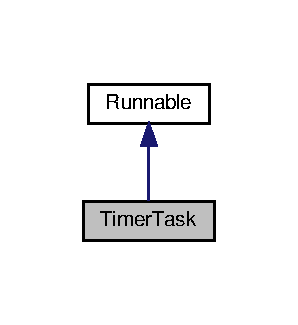
\includegraphics[width=143pt]{structTimerTask__inherit__graph}
\end{center}
\end{figure}


Timer\+Task 的协作图\+:\nopagebreak
\begin{figure}[H]
\begin{center}
\leavevmode
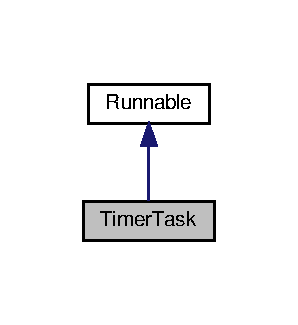
\includegraphics[width=143pt]{structTimerTask__coll__graph}
\end{center}
\end{figure}
\subsection*{Public 成员函数}
\begin{DoxyCompactItemize}
\item 
{\footnotesize template$<$typename F $>$ }\\\hyperlink{structTimerTask_ab87d7c5c62a8a079031b39eea3958c65}{Timer\+Task} (const std\+::chrono\+::nanoseconds \&init\+Delay, const std\+::chrono\+::nanoseconds \&interval, bool fixed\+Rate, F \&\&f)
\begin{DoxyCompactList}\small\item\em \hyperlink{structTimerTask}{Timer\+Task} 构造函数 \end{DoxyCompactList}\item 
\hyperlink{structTimerTask_a1b24917388958b16efb2d4d42593e96e}{Timer\+Task} (const \hyperlink{structTimerTask}{Timer\+Task} \&rh)
\begin{DoxyCompactList}\small\item\em \hyperlink{structTimerTask}{Timer\+Task} 拷贝构造 \end{DoxyCompactList}\item 
\mbox{\Hypertarget{structTimerTask_a028f1f4221afe88383ac3c17b4c1ea41}\label{structTimerTask_a028f1f4221afe88383ac3c17b4c1ea41}} 
\hyperlink{structTimerTask_a028f1f4221afe88383ac3c17b4c1ea41}{Timer\+Task} ()=default
\begin{DoxyCompactList}\small\item\em \hyperlink{structTimerTask}{Timer\+Task} 默认构造 \end{DoxyCompactList}\item 
\hyperlink{structTimerTask}{Timer\+Task} \& \hyperlink{structTimerTask_a3dfbb5770a1e3496f4e34d0795565c79}{operator=} (const \hyperlink{structTimerTask}{Timer\+Task} \&rh)
\begin{DoxyCompactList}\small\item\em operator= 赋值运算符 \end{DoxyCompactList}\end{DoxyCompactItemize}
\subsection*{Public 属性}
\begin{DoxyCompactItemize}
\item 
\mbox{\Hypertarget{structTimerTask_af49a805f814a0b92e1f96037226a2d2e}\label{structTimerTask_af49a805f814a0b92e1f96037226a2d2e}} 
std\+::chrono\+::nanoseconds \hyperlink{structTimerTask_af49a805f814a0b92e1f96037226a2d2e}{initial\+Delay\+\_\+} \{0\}
\begin{DoxyCompactList}\small\item\em 初次延迟 \end{DoxyCompactList}\item 
\mbox{\Hypertarget{structTimerTask_afd954f592d96d8abe152e0f54b30979e}\label{structTimerTask_afd954f592d96d8abe152e0f54b30979e}} 
std\+::chrono\+::nanoseconds \hyperlink{structTimerTask_afd954f592d96d8abe152e0f54b30979e}{interval\+\_\+} \{0\}
\begin{DoxyCompactList}\small\item\em 固定延迟或间隔 \end{DoxyCompactList}\item 
\mbox{\Hypertarget{structTimerTask_a31da300c15d00f58c2950e9752027e42}\label{structTimerTask_a31da300c15d00f58c2950e9752027e42}} 
bool \hyperlink{structTimerTask_a31da300c15d00f58c2950e9752027e42}{fixed\+Rate\+\_\+}
\begin{DoxyCompactList}\small\item\em 是否是固定间隔执行 \end{DoxyCompactList}\item 
\mbox{\Hypertarget{structTimerTask_a7bcf4dfd5b91038d4c4c5378285d4ed0}\label{structTimerTask_a7bcf4dfd5b91038d4c4c5378285d4ed0}} 
std\+::chrono\+::steady\+\_\+clock\+::time\+\_\+point \hyperlink{structTimerTask_a7bcf4dfd5b91038d4c4c5378285d4ed0}{call\+Time\+\_\+}
\begin{DoxyCompactList}\small\item\em 下次执行时间 \end{DoxyCompactList}\end{DoxyCompactItemize}
\subsection*{额外继承的成员函数}


\subsection{详细描述}
定时任务封装 

\subsection{构造及析构函数说明}
\mbox{\Hypertarget{structTimerTask_ab87d7c5c62a8a079031b39eea3958c65}\label{structTimerTask_ab87d7c5c62a8a079031b39eea3958c65}} 
\index{Timer\+Task@{Timer\+Task}!Timer\+Task@{Timer\+Task}}
\index{Timer\+Task@{Timer\+Task}!Timer\+Task@{Timer\+Task}}
\subsubsection{\texorpdfstring{Timer\+Task()}{TimerTask()}\hspace{0.1cm}{\footnotesize\ttfamily [1/2]}}
{\footnotesize\ttfamily template$<$typename F $>$ \\
Timer\+Task\+::\+Timer\+Task (\begin{DoxyParamCaption}\item[{const std\+::chrono\+::nanoseconds \&}]{init\+Delay,  }\item[{const std\+::chrono\+::nanoseconds \&}]{interval,  }\item[{bool}]{fixed\+Rate,  }\item[{F \&\&}]{f }\end{DoxyParamCaption})\hspace{0.3cm}{\ttfamily [inline]}}



\hyperlink{structTimerTask}{Timer\+Task} 构造函数 


\begin{DoxyParams}{参数}
{\em init\+Delay} & 第一次调用的延迟 \\
\hline
{\em interval} & 每次调用间隔 \\
\hline
{\em fixed\+Rate} & 是否等间隔运行,true执行间隔确定,false每次调用经过相同延迟 \\
\hline
{\em f} & lambda或\+Runnable \\
\hline
\end{DoxyParams}
\mbox{\Hypertarget{structTimerTask_a1b24917388958b16efb2d4d42593e96e}\label{structTimerTask_a1b24917388958b16efb2d4d42593e96e}} 
\index{Timer\+Task@{Timer\+Task}!Timer\+Task@{Timer\+Task}}
\index{Timer\+Task@{Timer\+Task}!Timer\+Task@{Timer\+Task}}
\subsubsection{\texorpdfstring{Timer\+Task()}{TimerTask()}\hspace{0.1cm}{\footnotesize\ttfamily [2/2]}}
{\footnotesize\ttfamily Timer\+Task\+::\+Timer\+Task (\begin{DoxyParamCaption}\item[{const \hyperlink{structTimerTask}{Timer\+Task} \&}]{rh }\end{DoxyParamCaption})\hspace{0.3cm}{\ttfamily [inline]}}



\hyperlink{structTimerTask}{Timer\+Task} 拷贝构造 


\begin{DoxyParams}{参数}
{\em rh} & 另一个\+Timer\+Task \\
\hline
\end{DoxyParams}


\subsection{成员函数说明}
\mbox{\Hypertarget{structTimerTask_a3dfbb5770a1e3496f4e34d0795565c79}\label{structTimerTask_a3dfbb5770a1e3496f4e34d0795565c79}} 
\index{Timer\+Task@{Timer\+Task}!operator=@{operator=}}
\index{operator=@{operator=}!Timer\+Task@{Timer\+Task}}
\subsubsection{\texorpdfstring{operator=()}{operator=()}}
{\footnotesize\ttfamily \hyperlink{structTimerTask}{Timer\+Task}\& Timer\+Task\+::operator= (\begin{DoxyParamCaption}\item[{const \hyperlink{structTimerTask}{Timer\+Task} \&}]{rh }\end{DoxyParamCaption})\hspace{0.3cm}{\ttfamily [inline]}}



operator= 赋值运算符 


\begin{DoxyParams}{参数}
{\em rh} & 另一个\+Timer\+Task\\
\hline
\end{DoxyParams}
\begin{DoxyReturn}{返回}
\hyperlink{structTimerTask}{Timer\+Task}\& 
\end{DoxyReturn}


该结构体的文档由以下文件生成\+:\begin{DoxyCompactItemize}
\item 
scheduledthreadpoolexecutor.\+hpp\end{DoxyCompactItemize}

\hypertarget{classWorkStealingThreadPoolExecutor}{}\section{Work\+Stealing\+Thread\+Pool\+Executor类 参考}
\label{classWorkStealingThreadPoolExecutor}\index{Work\+Stealing\+Thread\+Pool\+Executor@{Work\+Stealing\+Thread\+Pool\+Executor}}


任务窃取线程池,从下一个线程的任务队列窃取任务  




{\ttfamily \#include $<$workstealingthreadpoolexecutor.\+hpp$>$}



类 Work\+Stealing\+Thread\+Pool\+Executor 继承关系图\+:\nopagebreak
\begin{figure}[H]
\begin{center}
\leavevmode
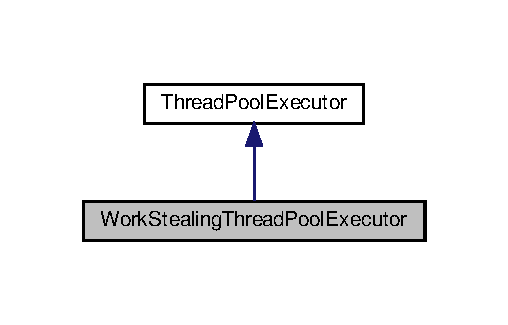
\includegraphics[width=244pt]{classWorkStealingThreadPoolExecutor__inherit__graph}
\end{center}
\end{figure}


Work\+Stealing\+Thread\+Pool\+Executor 的协作图\+:\nopagebreak
\begin{figure}[H]
\begin{center}
\leavevmode
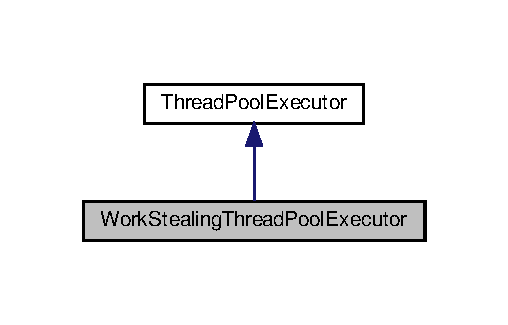
\includegraphics[width=244pt]{classWorkStealingThreadPoolExecutor__coll__graph}
\end{center}
\end{figure}
\subsection*{Public 成员函数}
\begin{DoxyCompactItemize}
\item 
\hyperlink{classWorkStealingThreadPoolExecutor_a3e4e9fd05b5b325f2f051725410525cb}{Work\+Stealing\+Thread\+Pool\+Executor} (int32\+\_\+t core\+Pool\+Size, int32\+\_\+t max\+Pool\+Size, const std\+::vector$<$ \hyperlink{classBlockingQueue}{Blocking\+Queue}$<$ \hyperlink{classRunnable_abe8d3066c7305401d6f0aad8e70780f2}{Runnable\+::sptr} $>$$>$ \&work\+Queue, const \hyperlink{classRejectedExecutionHandler}{Rejected\+Execution\+Handler} \&handler, const std\+::string \&prefix=\char`\"{}\char`\"{})
\begin{DoxyCompactList}\small\item\em \hyperlink{classWorkStealingThreadPoolExecutor}{Work\+Stealing\+Thread\+Pool\+Executor} 构造函数 \end{DoxyCompactList}\item 
\hyperlink{classWorkStealingThreadPoolExecutor_a80c8e32259e498cbb2c5625b272d37f3}{Work\+Stealing\+Thread\+Pool\+Executor} (int32\+\_\+t core\+Pool\+Size, int32\+\_\+t max\+Pool\+Size, const std\+::vector$<$ \hyperlink{classBlockingQueue}{Blocking\+Queue}$<$ \hyperlink{classRunnable_abe8d3066c7305401d6f0aad8e70780f2}{Runnable\+::sptr} $>$$>$ \&work\+Queue, \hyperlink{classRejectedExecutionHandler}{Rejected\+Execution\+Handler} $\ast$handler, const std\+::string \&prefix=\char`\"{}\char`\"{})
\begin{DoxyCompactList}\small\item\em \hyperlink{classWorkStealingThreadPoolExecutor}{Work\+Stealing\+Thread\+Pool\+Executor} 构造函数 \end{DoxyCompactList}\item 
\hyperlink{classWorkStealingThreadPoolExecutor_adb702388a229cc2a0508901976dd9104}{Work\+Stealing\+Thread\+Pool\+Executor} (int32\+\_\+t core\+Pool\+Size, int32\+\_\+t max\+Pool\+Size, const std\+::string \&prefix=\char`\"{}\char`\"{})
\begin{DoxyCompactList}\small\item\em \hyperlink{classWorkStealingThreadPoolExecutor}{Work\+Stealing\+Thread\+Pool\+Executor} 构造函数 \end{DoxyCompactList}\item 
{\footnotesize template$<$typename F $>$ }\\std\+::future$<$ typename std\+::result\+\_\+of$<$ F()$>$\+::type $>$ \hyperlink{classWorkStealingThreadPoolExecutor_a7fa1b79c8be2b06a7952ccfd14aa7f6c}{submit} (F f, bool core=true)
\begin{DoxyCompactList}\small\item\em submit 在将来某个时候执行给定的任务, 任务可以在新线程或现有的合并的线程中执行, 可以有返回值,向任务队列提交的是任务副本 会抛出异常 \end{DoxyCompactList}\item 
virtual void \hyperlink{classWorkStealingThreadPoolExecutor_ab0414f5e006e8fc523bfd35ba276f705}{worker\+Thread} (size\+\_\+t queue\+Idex) override
\begin{DoxyCompactList}\small\item\em worker\+Thread 核心工作线程 \end{DoxyCompactList}\item 
virtual void \hyperlink{classWorkStealingThreadPoolExecutor_ae4170b80bdc4ec806ee4a04cc5daaada}{core\+Worker\+Thread} (size\+\_\+t queue\+Idex) override
\begin{DoxyCompactList}\small\item\em worker\+Thread 非核心工作线程 \end{DoxyCompactList}\end{DoxyCompactItemize}
\subsection*{额外继承的成员函数}


\subsection{详细描述}
任务窃取线程池,从下一个线程的任务队列窃取任务 

\subsection{构造及析构函数说明}
\mbox{\Hypertarget{classWorkStealingThreadPoolExecutor_a3e4e9fd05b5b325f2f051725410525cb}\label{classWorkStealingThreadPoolExecutor_a3e4e9fd05b5b325f2f051725410525cb}} 
\index{Work\+Stealing\+Thread\+Pool\+Executor@{Work\+Stealing\+Thread\+Pool\+Executor}!Work\+Stealing\+Thread\+Pool\+Executor@{Work\+Stealing\+Thread\+Pool\+Executor}}
\index{Work\+Stealing\+Thread\+Pool\+Executor@{Work\+Stealing\+Thread\+Pool\+Executor}!Work\+Stealing\+Thread\+Pool\+Executor@{Work\+Stealing\+Thread\+Pool\+Executor}}
\subsubsection{\texorpdfstring{Work\+Stealing\+Thread\+Pool\+Executor()}{WorkStealingThreadPoolExecutor()}\hspace{0.1cm}{\footnotesize\ttfamily [1/3]}}
{\footnotesize\ttfamily Work\+Stealing\+Thread\+Pool\+Executor\+::\+Work\+Stealing\+Thread\+Pool\+Executor (\begin{DoxyParamCaption}\item[{int32\+\_\+t}]{core\+Pool\+Size,  }\item[{int32\+\_\+t}]{max\+Pool\+Size,  }\item[{const std\+::vector$<$ \hyperlink{classBlockingQueue}{Blocking\+Queue}$<$ \hyperlink{classRunnable_abe8d3066c7305401d6f0aad8e70780f2}{Runnable\+::sptr} $>$$>$ \&}]{work\+Queue,  }\item[{const \hyperlink{classRejectedExecutionHandler}{Rejected\+Execution\+Handler} \&}]{handler,  }\item[{const std\+::string \&}]{prefix = {\ttfamily \char`\"{}\char`\"{}} }\end{DoxyParamCaption})}



\hyperlink{classWorkStealingThreadPoolExecutor}{Work\+Stealing\+Thread\+Pool\+Executor} 构造函数 


\begin{DoxyParams}{参数}
{\em core\+Pool\+Size} & 核心线程数量 \\
\hline
{\em max\+Pool\+Size} & 最大线程数 \\
\hline
{\em work\+Queue} & 任务队列 \\
\hline
{\em handler} & 拒绝策略 \\
\hline
{\em prefix} & 线程名前缀 \\
\hline
\end{DoxyParams}
\mbox{\Hypertarget{classWorkStealingThreadPoolExecutor_a80c8e32259e498cbb2c5625b272d37f3}\label{classWorkStealingThreadPoolExecutor_a80c8e32259e498cbb2c5625b272d37f3}} 
\index{Work\+Stealing\+Thread\+Pool\+Executor@{Work\+Stealing\+Thread\+Pool\+Executor}!Work\+Stealing\+Thread\+Pool\+Executor@{Work\+Stealing\+Thread\+Pool\+Executor}}
\index{Work\+Stealing\+Thread\+Pool\+Executor@{Work\+Stealing\+Thread\+Pool\+Executor}!Work\+Stealing\+Thread\+Pool\+Executor@{Work\+Stealing\+Thread\+Pool\+Executor}}
\subsubsection{\texorpdfstring{Work\+Stealing\+Thread\+Pool\+Executor()}{WorkStealingThreadPoolExecutor()}\hspace{0.1cm}{\footnotesize\ttfamily [2/3]}}
{\footnotesize\ttfamily Work\+Stealing\+Thread\+Pool\+Executor\+::\+Work\+Stealing\+Thread\+Pool\+Executor (\begin{DoxyParamCaption}\item[{int32\+\_\+t}]{core\+Pool\+Size,  }\item[{int32\+\_\+t}]{max\+Pool\+Size,  }\item[{const std\+::vector$<$ \hyperlink{classBlockingQueue}{Blocking\+Queue}$<$ \hyperlink{classRunnable_abe8d3066c7305401d6f0aad8e70780f2}{Runnable\+::sptr} $>$$>$ \&}]{work\+Queue,  }\item[{\hyperlink{classRejectedExecutionHandler}{Rejected\+Execution\+Handler} $\ast$}]{handler,  }\item[{const std\+::string \&}]{prefix = {\ttfamily \char`\"{}\char`\"{}} }\end{DoxyParamCaption})}



\hyperlink{classWorkStealingThreadPoolExecutor}{Work\+Stealing\+Thread\+Pool\+Executor} 构造函数 


\begin{DoxyParams}{参数}
{\em core\+Pool\+Size} & 核心线程数量 \\
\hline
{\em max\+Pool\+Size} & 最大线程数 \\
\hline
{\em work\+Queue} & 任务队列 \\
\hline
{\em handler} & 拒绝策略 \\
\hline
{\em prefix} & 线程名前缀 \\
\hline
\end{DoxyParams}
\mbox{\Hypertarget{classWorkStealingThreadPoolExecutor_adb702388a229cc2a0508901976dd9104}\label{classWorkStealingThreadPoolExecutor_adb702388a229cc2a0508901976dd9104}} 
\index{Work\+Stealing\+Thread\+Pool\+Executor@{Work\+Stealing\+Thread\+Pool\+Executor}!Work\+Stealing\+Thread\+Pool\+Executor@{Work\+Stealing\+Thread\+Pool\+Executor}}
\index{Work\+Stealing\+Thread\+Pool\+Executor@{Work\+Stealing\+Thread\+Pool\+Executor}!Work\+Stealing\+Thread\+Pool\+Executor@{Work\+Stealing\+Thread\+Pool\+Executor}}
\subsubsection{\texorpdfstring{Work\+Stealing\+Thread\+Pool\+Executor()}{WorkStealingThreadPoolExecutor()}\hspace{0.1cm}{\footnotesize\ttfamily [3/3]}}
{\footnotesize\ttfamily Work\+Stealing\+Thread\+Pool\+Executor\+::\+Work\+Stealing\+Thread\+Pool\+Executor (\begin{DoxyParamCaption}\item[{int32\+\_\+t}]{core\+Pool\+Size,  }\item[{int32\+\_\+t}]{max\+Pool\+Size,  }\item[{const std\+::string \&}]{prefix = {\ttfamily \char`\"{}\char`\"{}} }\end{DoxyParamCaption})}



\hyperlink{classWorkStealingThreadPoolExecutor}{Work\+Stealing\+Thread\+Pool\+Executor} 构造函数 


\begin{DoxyParams}{参数}
{\em core\+Pool\+Size} & 核心线程数量 \\
\hline
{\em max\+Pool\+Size} & 最大线程数 \\
\hline
{\em prefix} & 线程名前缀 \\
\hline
\end{DoxyParams}


\subsection{成员函数说明}
\mbox{\Hypertarget{classWorkStealingThreadPoolExecutor_ae4170b80bdc4ec806ee4a04cc5daaada}\label{classWorkStealingThreadPoolExecutor_ae4170b80bdc4ec806ee4a04cc5daaada}} 
\index{Work\+Stealing\+Thread\+Pool\+Executor@{Work\+Stealing\+Thread\+Pool\+Executor}!core\+Worker\+Thread@{core\+Worker\+Thread}}
\index{core\+Worker\+Thread@{core\+Worker\+Thread}!Work\+Stealing\+Thread\+Pool\+Executor@{Work\+Stealing\+Thread\+Pool\+Executor}}
\subsubsection{\texorpdfstring{core\+Worker\+Thread()}{coreWorkerThread()}}
{\footnotesize\ttfamily virtual void Work\+Stealing\+Thread\+Pool\+Executor\+::core\+Worker\+Thread (\begin{DoxyParamCaption}\item[{size\+\_\+t}]{queue\+Idex }\end{DoxyParamCaption})\hspace{0.3cm}{\ttfamily [override]}, {\ttfamily [virtual]}}



worker\+Thread 非核心工作线程 


\begin{DoxyParams}{参数}
{\em queue\+Idex} & 线程队列位置 \\
\hline
\end{DoxyParams}


重载 \hyperlink{classThreadPoolExecutor_a5e40839bf4191b5eab9d81227ddb62c3}{Thread\+Pool\+Executor} .

\mbox{\Hypertarget{classWorkStealingThreadPoolExecutor_a7fa1b79c8be2b06a7952ccfd14aa7f6c}\label{classWorkStealingThreadPoolExecutor_a7fa1b79c8be2b06a7952ccfd14aa7f6c}} 
\index{Work\+Stealing\+Thread\+Pool\+Executor@{Work\+Stealing\+Thread\+Pool\+Executor}!submit@{submit}}
\index{submit@{submit}!Work\+Stealing\+Thread\+Pool\+Executor@{Work\+Stealing\+Thread\+Pool\+Executor}}
\subsubsection{\texorpdfstring{submit()}{submit()}}
{\footnotesize\ttfamily template$<$typename F $>$ \\
std\+::future$<$typename std\+::result\+\_\+of$<$F()$>$\+::type$>$ Work\+Stealing\+Thread\+Pool\+Executor\+::submit (\begin{DoxyParamCaption}\item[{F}]{f,  }\item[{bool}]{core = {\ttfamily true} }\end{DoxyParamCaption})\hspace{0.3cm}{\ttfamily [inline]}}



submit 在将来某个时候执行给定的任务, 任务可以在新线程或现有的合并的线程中执行, 可以有返回值,向任务队列提交的是任务副本 会抛出异常 


\begin{DoxyParams}{参数}
{\em f} & 要提交的任务(Runnable或函数或lambda) \\
\hline
{\em core} & 是否使用核心线程(默认值true,不增加新线程)\\
\hline
\end{DoxyParams}
\begin{DoxyReturn}{返回}
res 任务返回值的future 
\end{DoxyReturn}
\mbox{\Hypertarget{classWorkStealingThreadPoolExecutor_ab0414f5e006e8fc523bfd35ba276f705}\label{classWorkStealingThreadPoolExecutor_ab0414f5e006e8fc523bfd35ba276f705}} 
\index{Work\+Stealing\+Thread\+Pool\+Executor@{Work\+Stealing\+Thread\+Pool\+Executor}!worker\+Thread@{worker\+Thread}}
\index{worker\+Thread@{worker\+Thread}!Work\+Stealing\+Thread\+Pool\+Executor@{Work\+Stealing\+Thread\+Pool\+Executor}}
\subsubsection{\texorpdfstring{worker\+Thread()}{workerThread()}}
{\footnotesize\ttfamily virtual void Work\+Stealing\+Thread\+Pool\+Executor\+::worker\+Thread (\begin{DoxyParamCaption}\item[{size\+\_\+t}]{queue\+Idex }\end{DoxyParamCaption})\hspace{0.3cm}{\ttfamily [override]}, {\ttfamily [virtual]}}



worker\+Thread 核心工作线程 


\begin{DoxyParams}{参数}
{\em queue\+Idex} & 线程队列位置 \\
\hline
\end{DoxyParams}


重载 \hyperlink{classThreadPoolExecutor_a844902ce61fb16b11a569b8ee56e80e9}{Thread\+Pool\+Executor} .



该类的文档由以下文件生成\+:\begin{DoxyCompactItemize}
\item 
workstealingthreadpoolexecutor.\+hpp\end{DoxyCompactItemize}

%--- End generated contents ---

% Index
\backmatter
\newpage
\phantomsection
\clearemptydoublepage
\addcontentsline{toc}{chapter}{索引}
\printindex

\end{document}
